% 中文实证工作稿，更新：2026-10-08；使用 XeLaTeX 编译两遍。
% 数据依据：experiments/EXPERIMENT_PLAN_20261008.md
% 图表来源：papers/figures/pilot_20261008/manifest.json
% 两 seed CUDA pilot，加固定完整 trace 池的 CPU 机制实验；不把后者当 GPU 测量。
\documentclass[11pt,twocolumn]{ctexart}
\usepackage[margin=1in]{geometry}
\usepackage{amsmath,amssymb}
\usepackage{graphicx}
\usepackage{booktabs}
\usepackage[hidelinks]{hyperref}
\usepackage{enumitem}
\usepackage{array}
\usepackage{algorithm}
\usepackage{algpseudocode}
\IfFileExists{placeins.sty}{\usepackage{placeins}}{\newcommand{\FloatBarrier}{\clearpage}}
\emergencystretch=3em
\newcommand{\pending}{\textit{待测}}
\newcommand{\plannedpanel}[2]{%
  \fbox{\begin{minipage}[c][#1][c]{\dimexpr\linewidth-2\fboxsep-2\fboxrule\relax}
  \centering\small\textbf{待补实验}\par\medskip #2
  \end{minipage}}}

\title{\bfseries Scout：约束引导采样与分级筛选的张量程序自动搜索调优}
\author{作者姓名 \\ \small 单位}
\date{}
\begin{document}
\maketitle

\begin{abstract}
张量程序是实现矩阵乘、卷积和归约等深度学习算子的基础，其执行性能直接影响模型推理效率。通过调优循环切分、数据布局和并行映射等调度决策，可以改善目标硬件的资源利用，因此张量程序调优是提升深度学习计算性能的关键环节。目前，以 Ansor 和 MetaSchedule 为代表的基于搜索的自动调优方法已得到广泛应用，但仍面临候选空间庞大、搜索效率低和调优成本高等问题。针对上述问题，本文提出约束引导的张量程序自动调优框架 Scout，将硬件约束与分级筛选相结合，从搜索空间约束和候选评估两个方面减少无效探索与评估开销，提高有限测量预算下的搜索效率。我们将 Scout 集成到 TVM 编译器中，并在矩阵乘、卷积和归约等典型算子上开展实验。实验结果表明，Scout 的剪枝配置在达到基线搜索终点的延迟目标时取得最高 1.99 倍的调优加速，对应耗时减少 49.7\%；分级筛选配置相较剪枝配置，将学习代价模型评分耗时最高降低 91.4\%。
\end{abstract}

\section{引言}
\label{sec:intro}
深度学习加速器（GPU、NPU 等）推动了深度神经网络在自动驾驶、增强现实等领域的广泛应用。为提升模型推理速度，张量程序优化已成为最大化硬件计算效率的关键环节。现有深度学习框架将网络表示为计算图（节点对应卷积、矩阵乘等算子），并把算子映射到针对特定硬件手工优化的算子库（如 cuDNN、MKL-DNN）。然而，针对每类硬件、每个算子手工调优算子库，需要极强的专业知识和巨大的人力投入，严重阻碍了新型算子与定制化硬件的高效开发与迭代。

基于搜索的深度学习编译器（如 Ansor、MetaSchedule）是近年来更具扩展性的自动化方案。针对给定算子，它定义一个调度搜索空间，从中搜索适配目标硬件的最优编译后张量程序；搜索过程的核心是代价模型，用于预估候选程序的性能，从而减少耗时的硬件实测环节。

随着调度空间规模与算子种类的增长，基于搜索的编译器面临以下挑战：

第一，\textbf{搜索探索机制效率低下}。现有流程在采样、回放与验证之后才发现大量候选违反资源约束，将计算消耗在最终被丢弃的非法候选上。在本文的基线测量中，约 $80\%$ 的生成候选在经历回放、后处理与 lowering 之后才被 VerifyGPUCode 拒绝。

第二，\textbf{可学习代价模型导致搜索过程耗时}。现有方法在进化循环内的打分阶段，对所有候选逐一调用可学习代价模型、提取特征并完成推理，带来高昂的推理耗时与推理开销，成本远高于固定解析公式，使搜索过程耗时长。

针对上述问题，本文提出“剪枝+分级筛选”的约束引导搜索框架。剪枝即空间剪枝，把可证明的线程契约判定前移到采样与回放阶段：约束引导采样（CS）在采样决策点枚举并剔除必然违反线程契约的决策，从源头减少非法候选；分层硬筛（H）在回放前后对候选做线程判定，拦截可证明违规的候选，二者共同优化搜索空间、提高有效候选占比。分级筛选让代价模型不再参与进化迭代，而是分级评分——先用廉价的解析评分对候选初次粗筛，迭代结束后再用代价模型对入围候选细筛，从而加速调度搜索流程。

我们将 Scout 集成进 TVM 编译器，并在 MatMul128/256、标准卷积与大归约等算子上开展实验。结果表明，剪枝将候选生成次数减少约 62\%、Verify 失败减少约 85\%，有效候选占比由约 24\% 提升到约 70\%；分级筛让进化循环内不再调用代价模型，大幅削减了代价模型推理开销（数值留白待补）。多模型、端到端与多轮调优的实验结果显示（留白待补）。

本文的主要贡献可总结如下：
\begin{itemize}[leftmargin=1.6em]
\item \textbf{约束引导的搜索框架。}将可证明的线程约束判定前移，根据硬件参数（线程契约、每块线程上限、warp size）动态调整搜索空间，在采样决策点与回放阶段剪除违反约束的候选，从源头减少非法候选、提高剪枝有效性。
\item \textbf{分级筛选。}在进化迭代中以基于硬件参数的轻量解析评分对候选粗筛打分，再由学习代价模型对入围候选做二级精筛，在加快调优速度的同时保持调优效果，并降低代价模型的训练复杂度。
\end{itemize}

\section{背景}
\label{sec:background}

\subsection{张量程序调优}
深度学习模型的推理性能由两个层面的优化共同决定：一是图级优化，即在计算图上做算子融合、常量折叠、量化等变换；二是算子级优化，即对卷积、矩阵乘、归约等张量算子做面向硬件的调度优化，这正是张量程序调优的核心。张量程序的性能由循环切分、线程与寄存器绑定、向量化、数据复用与缓存放置等调度决策决定，同一算子在相同硬件上因调度不同、性能可相差数十倍。

张量程序调优的做法大致经历三个阶段。最传统的是手工调优：由专家针对特定硬件手写高性能算子库（如 cuDNN、cuBLAS、MKL-DNN），性能最优但人力成本极高、难以扩展到新算子与新硬件。随后出现基于领域专用语言的模板方法：Halide~\cite{halide} 首次把算法与调度解耦，让开发者以独立于算法的语言描述并行、局部性与向量化；TVM~\cite{tvm} 将这一思想推广到深度学习算子，引入 \texttt{split}、\texttt{reorder}、\texttt{bind} 等调度原语与张量化，但编写高效模板仍依赖专家经验。

这促使自动化调优的兴起：把“写调度”变为“搜调度”，由编译器在预定义的调度搜索空间中自动寻找最优调度，并用代价模型指导搜索、减少昂贵的硬件实测。

\subsection{基于搜索的AI编译器}
基于搜索的编译器是自动化调优的代表性实现，主流系统在搜索空间的表达方式与搜索策略上各有侧重。多面体编译（如 Tiramisu~\cite{tiramisu}、Tensor Comprehensions）把循环变换建模为整数仿射变换，在多面体模型上枚举合法的变换组合，可系统化地搜索并行与局部性优化，但对非规则控制流与复杂访存支持有限。TVM~\cite{tvm} 的 AutoTVM 采用“模板 + 学习代价模型”：模板定义候选实现的合法调度集合，代价模型（如 XGBoost）预估性能、以贝叶斯或遗传搜索挑选候选。Ansor~\cite{ansor} 去掉手工模板、用分层搜索空间（sketch 与 annotation）覆盖更广的调度。MetaSchedule~\cite{metaschedule} 用概率程序表达调度规则，把采样、变异与进化搜索统一。Triton~\cite{triton} 面向 GPU 提供类 Python 的块级编程接口，把块内调度交给编译器自动生成，兼顾可编程性与自动优化。本文的工作建立在 MetaSchedule 之上，其搜索流水线为：调度规则采样生成候选，经回放与后处理构造 S-TIR，\texttt{VerifyGPUCode} 验证资源合法性，再由学习代价模型打分、进化搜索择优，少量候选经 \emph{Builder} 编译、\emph{Runner} 实测并回填代价模型，整体工作流如图~\ref{fig:tuning-landscape} 所示。

\begin{figure}[tb]
\centering
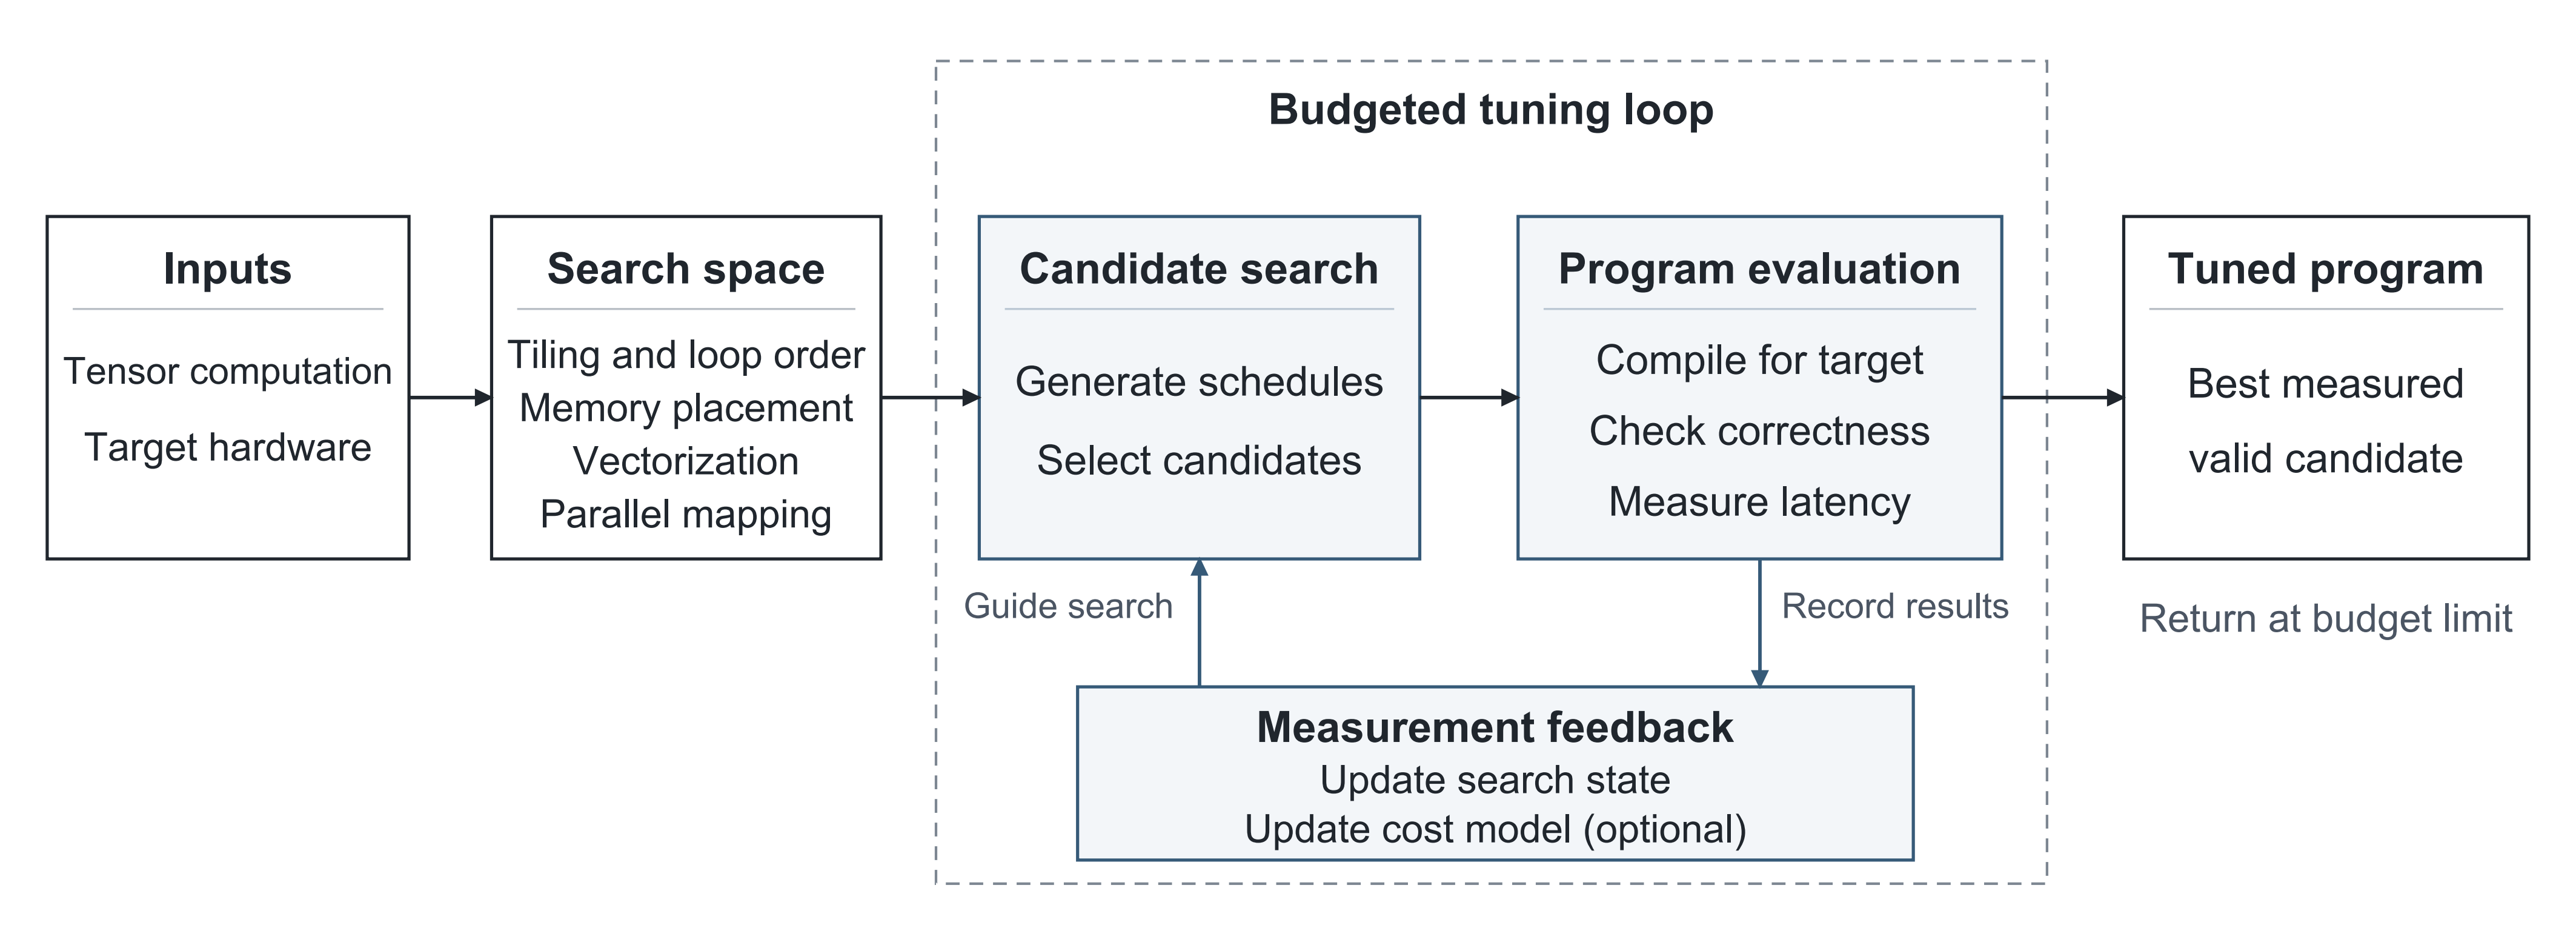
\includegraphics[width=\columnwidth]{figures/pilot_20261008/tensor_program_tuning.png}
\caption{张量程序自动调优工作流。张量计算与目标硬件共同确定调度搜索空间；预算受限的调优循环生成候选、编译验证并实测，用测量反馈更新搜索状态与代价模型，最终返回最佳实测的合法候选。}
\label{fig:tuning-landscape}
\end{figure}

\subsection{基于搜索技术的局限}
尽管基于搜索的编译器比手工调优更便捷，但针对每个新算子、每类新硬件往往需要重新搜索、难以泛化，且搜索效率仍面临三方面局限。其一，搜索空间有效候选少：仅 MatMul $128^3$ 的 \texttt{SamplePerfectTile} 因式分解就有数百万种组合，其中绝大多数违反硬件资源约束。其二，失败大多集中在事前的浪费：候选直到回放与 lowering 验证之后才被判非法，无效候选在昂贵的后期阶段才被丢弃。其三，代价模型更迭成本高：进化搜索的每一代都要对种群调用学习代价模型，特征提取与推理开销随候选规模增长，且模型需要反复训练。

表~\ref{tab:invalid-ratio} 报告了一次基线搜索的候选去向：约 $81\%$ 的生成候选最终被 \texttt{VerifyGPUCode} 拒绝，其中约 $91\%$ 是线程契约违规，有效候选仅占约 $19\%$。综上，现有搜索技术的核心局限可归纳为三点：（1）搜索空间有效候选少；（2）失败大多集中在事前的浪费；（3）代价模型更迭成本高、在 GA 过程中训练复杂。这正是本文要解决的问题。

\begin{table}[tb]
\centering
\caption{Candidate outcomes of one baseline search (MatMul $128^3$, seed S31).}
\label{tab:invalid-ratio}
\begin{tabular}{lr}
\toprule
Outcome & Count \\
\midrule
Generated candidates & 1303 \\
Passed postprocessing & 243 \\
Rejected by VerifyGPUCode & 1060 \\
\quad Thread constraint & 970 \\
\quad Shared memory & 60 \\
\quad Lowering exception & 30 \\
\bottomrule
\end{tabular}
\end{table}

\section{方法}
\label{sec:design}

本文提出的系统整体流程如图~\ref{fig:architecture} 所示：首先通过剪枝约束搜索空间，在采样与回放阶段前移线程契约判定、减少非法候选；初始化得到合法候选种群后进入 GA 迭代优化候选，此过程中以解析评分对候选做粗排序、指导变异方向；迭代若干轮后，将候选交由学习代价模型做最终裁定评分，并选出少量候选上机编译实测。下面分别介绍剪枝与分级筛选两个核心组件。

\begin{figure*}[tb]
\centering
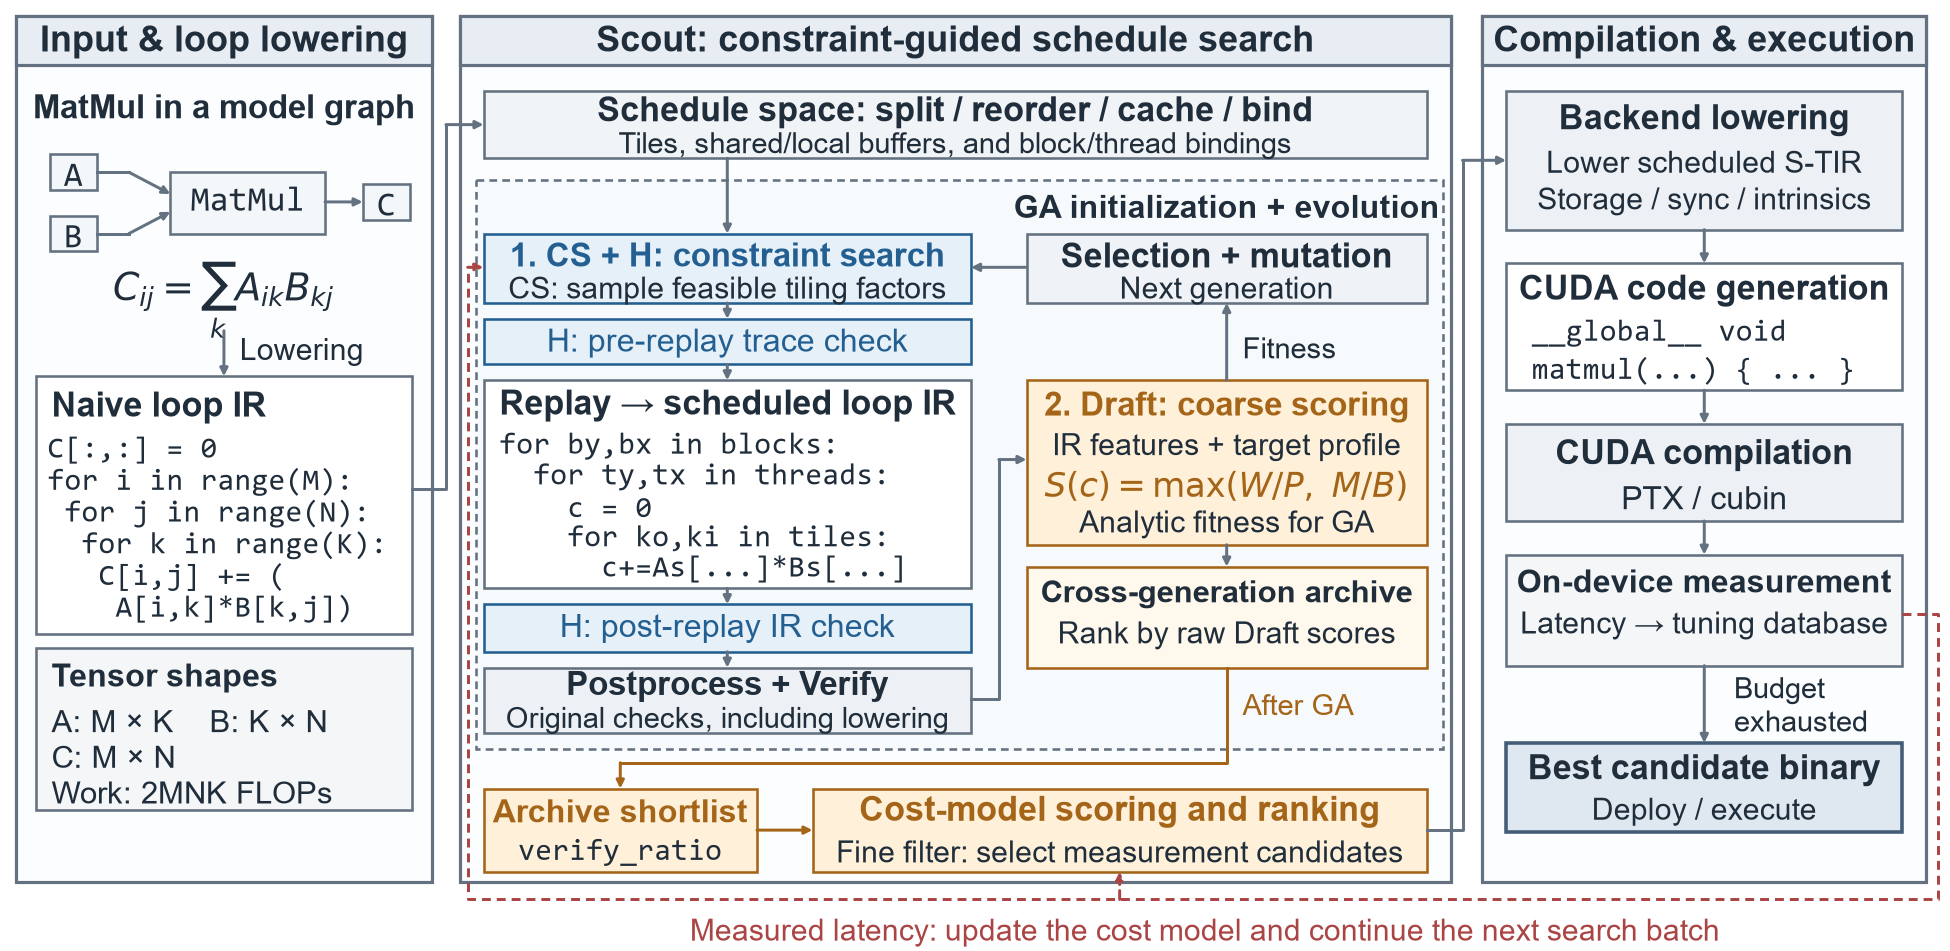
\includegraphics[width=\linewidth]{figures/architecture_matmul_wide/architecture_matmul.png}
\caption{系统整体架构。剪枝（CS+H）约束搜索空间、提高有效候选占比；初始化得到合法种群后进行 GA 迭代，以解析评分粗筛指导变异方向；批末由代价模型精筛排序，最终上机实测，实测反馈回更新代价模型。}
\label{fig:architecture}
\end{figure*}

\subsection{剪枝：约束引导采样与分层硬筛}
循环切分与线程绑定共同决定候选调度的并行配置。传统搜索先生成这些决策，再通过调度回放构造候选程序，最后由后处理检查其合法性。因此，即使线程配置已经超出设备限制，候选仍可能消耗完整的回放和验证开销。Scout 将线程约束前移到候选生成过程：约束引导采样（CS）在采样时缩小决策域，分层硬筛（H）在回放前后检查已有候选。二者共用硬件参数推导的线程约束，分别作用于新决策的生成与已有决策的筛选。

\paragraph{硬件约束表示}
对执行块 $b$，设三个线程维度的物理线程数分别为 $t_{b,x}$、$t_{b,y}$ 和 $t_{b,z}$，未使用的维度取 1，则每个线程块的线程数为
\begin{equation}
T_b=t_{b,x}t_{b,y}t_{b,z}.
\label{eq:thread-count}
\end{equation}
根据目标设备的线程块容量与 warp 宽度，结合算子的并行规模，确定可接受的线程数区间：
\begin{equation}
L_b\le T_b\le U_b,\qquad U_b=T_{\max}.
\label{eq:thread-range}
\end{equation}
其中，$T_{\max}$ 为设备允许的每块最大线程数；下限 $L_b$ 依据 warp 宽度确定，在并行规模充足时取一个 warp 的线程数，在较小计算规模下取 1。上限约束排除超出设备容量的配置，下限约束则限制并行规模充足时过小的线程配置。相关硬件参数及其作用见表~\ref{tab:target-attributes}。

\begin{table*}[tb]
\centering
\caption{线程剪枝及后续验证使用的硬件参数}
\label{tab:target-attributes}
\small
\setlength{\tabcolsep}{4pt}
\renewcommand{\arraystretch}{1.15}
\begin{tabular}{@{}lp{0.07\textwidth}p{0.24\textwidth}p{0.30\textwidth}@{}}
\toprule
目标属性 & 符号 & 含义（单位） & 方法中的作用 \\
\midrule
\texttt{max\_threads\_per\_block} & $T_{\max}$ & 每个线程块的最大线程数（线程） & 确定线程数上限，排除超出设备容量的配置 \\
\texttt{thread\_warp\_size} & $W_{\mathrm{warp}}$ & 每个 warp 的物理线程数（线程） & 结合并行规模确定线程数下限，并将 warp 级配置换算为物理线程数 \\
\texttt{max\_shared\_memory\_per\_block} & $S_{\max}$ & 每个线程块的共享内存容量（字节） & 在后续低层验证中检查候选程序的实际共享内存用量 \\
\bottomrule
\end{tabular}
\end{table*}

\paragraph{约束引导采样（CS）}
CS 从调度 trace 中分析采样决策与线程绑定的依赖关系。循环切分产生线程维度的长度，循环融合使多个长度相乘，因此可将维度 $d$ 的线程数表示为
\begin{equation}
t_{b,d}=C_{b,d}\prod_{f\in F_{b,d}}f,
\label{eq:thread-dim}
\end{equation}
其中 $C_{b,d}$ 是已知的常数部分，$F_{b,d}$ 是决定该维度长度的采样因子集合。该表示将线程约束转化为采样因子之间的约束，使候选无需完成回放即可接受检查。

在每个待采样位置，CS 首先构造满足原始调度规则的决策域，再结合已经确定的决策，保留满足式~\eqref{eq:thread-range} 的选项。例如，循环切分仍须满足各因子乘积等于原循环长度；线程约束进一步限制其中用于线程绑定的因子。随后，CS 从保留的决策中采样，并用该结果继续回放。循环切分在可行因子向量中均匀采样，类别选择则保留可行选项之间的相对概率。算法~\ref{alg:cs} 给出这一过程。若可行域为空，则重新尝试生成候选；重试次数受预设上限限制。

\paragraph{矩阵乘示例}
考虑 $C=AB$，其中 $A,B\in\mathbb{R}^{128\times128}$。将输出行循环切分为 $(i_0,i_1,i_2)$，满足 $i_0i_1i_2=128$，并将长度为 $i_2$ 的循环绑定到 \texttt{threadIdx.x}。若 \texttt{threadIdx.y} 已固定为 32 个线程，且未使用 $z$ 维，则 $T_b=32i_2$。在 $T_{\max}=1024$、$W_{\mathrm{warp}}=32$ 的设备上，该计算的线程数范围为 $[32,1024]$，从而要求 $i_2\le32$。因子 $i_2=64$ 和 $i_2=128$ 分别产生 2048 和 4096 个线程，均被 CS 从待采样域中排除；其余切分仍须满足原有因子乘积与切分规则。这样，已知的线程绑定直接约束后续决策，避免生成两维分别可选、组合后却超出线程块上限的配置。

\begin{algorithm}[!tb]
\caption{Constraint-guided sampling (CS)}
\label{alg:cs}
\small
\begin{algorithmic}[1]
\Require Trace $\tau$ and hardware parameters $\mathcal{H}$
\Ensure Replayed trace or a retry request
\State $P\gets\Call{BuildConstraints}{\tau,\mathcal{H}}$
\State Start replay with existing decisions fixed
\For{each unresolved sampling point $s$}
    \State $\pi\gets$ current replay prefix
    \State $D_s\gets\Call{OriginalDomain}{s}$
    \State $D_s^{+}\gets\Call{FilterDomain}{P,\pi,s,D_s}$
    \If{$D_s^{+}$ cannot be determined}
        \State $v\gets\Call{OriginalSample}{s}$
    \ElsIf{$D_s^{+}=\varnothing$}
        \State \Return \textsc{Retry}
    \Else
        \State $v\gets\Call{SampleFeasible}{D_s^{+},s}$
    \EndIf
    \State Record $v$ at $s$ and continue replay
\EndFor
\If{CS detects a thread-constraint violation}
    \State \Return \textsc{Retry}
\EndIf
\State \Return replayed trace
\end{algorithmic}
\end{algorithm}

\paragraph{分层硬筛（H）}
初始化与进化变异得到的候选可能已携带完整决策，无法仅靠约束后续采样排除。H 因此在两个阶段检查候选。首先，在 trace 层将已有决策代入线程表达式，提前拒绝能够确定违反约束的候选，省去其回放与后处理开销。随后，对保留候选完成回放，并在 IR 层根据实际线程绑定重新检查，阻止违规候选进入后续验证与编译。两层检查分别利用调度决策和生成程序中的信息，使同一组线程约束覆盖候选构造的不同阶段。

在上述矩阵乘示例中，若变异将 $i_2$ 改为 64，H 可在 trace 层根据 $32\times64>1024$ 直接拒绝该候选。CS 与 H 由此形成互补：前者限制新决策的取值，后者检查初始化及变异产生的已有决策。对于尚不能确定的线程配置，候选继续沿原流程接受检查；通过线程筛选的候选仍需完成原有后处理与 \texttt{VerifyGPUCode}，以验证共享内存等其他资源限制。

\subsection{分级筛选：粗筛与精筛}
剪枝减少了不可行候选，但进化搜索仍需在大量可行调度之间比较性能。若对每一代种群均调用学习代价模型，特征提取与预测便会反复作用于最终不会被测量的候选。Scout 采用两级评分：先用基于静态分析的 Draft 评分指导进化搜索，保留一组有潜力的候选，再由学习代价模型进行精筛，确定提交设备测量的方案。Draft 提供高频比较所需的低成本排序信号，学习代价模型则利用累积的实测反馈完成最终选拔。

\paragraph{候选特征与硬件参数}
Draft 采用 Pruner 的解析代价估计思路~\cite{pruner}，以完成回放和后处理的 S-TIR 为输入，从循环结构、缓冲区访问及线程绑定中提取候选特征。对候选 $c$，记其特征记录集合为 $\mathcal S(c)$。每条记录 $s$ 包含计算工作量 $W_s$、DRAM 访问量代理 $M_s$、数据复用因子 $R_s$、寄存器需求代理 $Q_s$，以及网格规模 $g_s$ 和块线程数 $t_s$。这些特征随切分、融合和线程映射等调度决策变化，用于刻画候选的工作量、数据访问与并行组织。

硬件参数为上述特征提供统一的评价尺度。峰值算力 $P$ 与内存带宽 $B$ 分别确定计算和访存项的基准；SM 数量 $n_{\mathrm{SM}}$、warp 宽度 $W_{\mathrm{warp}}$、每 SM 活动块参考数 $a$ 及 SM 分区数 $p$ 用于估计并行利用率；寄存器参考容量 $Q_{\mathrm{cap}}$ 用于归一化寄存器压力。这些参数由目标设备描述及预设硬件配置提供，在同一设备的搜索过程中保持固定。表~\ref{tab:analytic-params} 列出了各项输入的含义及作用。

\begin{table*}[tb]
\centering
\caption{Draft 评分使用的候选特征与硬件参数}
\label{tab:analytic-params}
\small
\setlength{\tabcolsep}{4pt}
\renewcommand{\arraystretch}{1.12}
\begin{tabular}{@{}p{0.14\textwidth}p{0.27\textwidth}p{0.54\textwidth}@{}}
\toprule
符号 & 含义 & 提取依据或评分作用 \\
\midrule
\multicolumn{3}{@{}l}{\textbf{候选静态特征}} \\
$W_s$ & 计算工作量 & 根据浮点运算、循环长度及线程映射估计，构成计算项的工作量输入 \\
$M_s$ & DRAM 访问量代理 & 根据访存语句、循环索引及存储作用域估计，构成访存项的输入 \\
$R_s$ & 数据复用因子 & 由线程内计算量与访问量的比例构造，用于修正数据复用对计算代价的影响 \\
$Q_s$ & 寄存器需求代理 & 根据访问索引涉及的循环规模估计，与 $Q_{\mathrm{cap}}$ 比较以刻画寄存器压力 \\
$g_s,\ t_s$ & 网格规模与块线程数 & 从物理线程绑定提取，用于估计调度波次、SM 并行度及 warp 填充程度 \\
\midrule
\multicolumn{3}{@{}l}{\textbf{硬件参数与参考配置}} \\
$P,\ B$ & 峰值算力与内存带宽 & 分别为计算工作量与访存量提供代价换算基准 \\
$n_{\mathrm{SM}}$ & SM 数量 & 确定设备可并行调度线程块的规模 \\
$W_{\mathrm{warp}}$ & warp 宽度 & 将块线程数换算为 warp 数，并估计未填满 warp 的利用率损失 \\
$a,\ p$ & 每 SM 活动块参考数与 SM 分区数 & 分别用于线程块调度容量和网格较小时的 SM 内并行度估计 \\
$Q_{\mathrm{cap}}$ & 寄存器参考容量 & 作为寄存器需求代理的归一化尺度，用于修正有效计算吞吐率 \\
\bottomrule
\end{tabular}
\end{table*}

\paragraph{Draft 解析评分}
Draft 分别估计每条特征记录的计算代价与访存代价，并以二者中的较大值刻画主要瓶颈。为考虑调度对计算资源利用的影响，定义有效计算吞吐率
\begin{equation}
P_s^{\mathrm{eff}}=
\frac{P\,\eta_s^{\mathrm{grid}}\eta_s^{\mathrm{warp}}}
{\max(1,Q_s/Q_{\mathrm{cap}})}.
\label{eq:draft-throughput}
\end{equation}
其中，$\eta_s^{\mathrm{grid}}$ 表示网格的并行利用率修正：当网格规模足以覆盖设备时，根据 $g_s$ 与 $n_{\mathrm{SM}}a$ 估计调度波次及末波填充程度；当网格较小时，则结合 $p$ 和每块 warp 数估计 SM 内的并行度。$\eta_s^{\mathrm{warp}}$ 表示已分配 warp 中有效线程所占的比例，由 $t_s$ 和 $W_{\mathrm{warp}}$ 确定。寄存器需求超过参考容量时，分母中的压力项降低有效吞吐率。

计算时间估计 $\widehat t_s^{\mathrm{comp}}$ 以 $W_s/P_s^{\mathrm{eff}}$ 为基础，并乘以复用修正项 $1+1/R_s$；复用因子越大，该项带来的额外代价越小。访存时间估计 $\widehat t_s^{\mathrm{mem}}$ 则由 $M_s$ 和带宽 $B$ 换算得到。这里的访存量与寄存器需求来自静态分析，分别作为内存流量和寄存器压力的代理。完成相应的尺度与单位换算后，候选的总估计代价及 Draft 分数为
\begin{equation}
\begin{aligned}
\widehat T(c)&=\sum_{s\in\mathcal S(c)}
\max\!\left(\widehat t_s^{\mathrm{comp}},\widehat t_s^{\mathrm{mem}}\right),\\
D(c)&=\frac{1}{\widehat T(c)}.
\end{aligned}
\label{eq:analytic}
\end{equation}
因此，较大的 $D(c)$ 表示较低的估计代价。Draft 无需利用测量样本训练，而是通过候选结构与固定硬件参数之间的关系比较调度方案。

以 MatMul $128^3$ 为例，若每个线程块计算一个输出 tile，将 tile 从 $16\times16$ 增大到 $32\times32$，网格规模便从 64 个块减为 16 个块。两种方案的计算总量相同，但较大的 tile 会改变块内数据复用和寄存器需求，同时减少可并行调度的线程块。Draft 将这些变化共同纳入评分，使切分方案的比较同时考虑数据复用与并行利用率。

\paragraph{Draft 引导的进化搜索}
在每个搜索批次内，Scout 建立大小为 $N$ 的初始种群，并执行 $G$ 轮进化。初始种群及各代子代均由 Draft 评分，同代分数经归一化后用于父代抽样。GA 对选中的父代调度进行变异，子代经过第 3.1 节的 CS 与 H，以及原有回放、后处理和验证后进入下一代。若在有限重试内无法生成可行子代，则保留父代。对于无法获得 Draft 分数的候选，保留较小的非零抽样权重；若整代均无法评分，则采用均匀抽样。

为保留早期种群中出现的优质候选，搜索同时维护跨代候选池 $A$。设本批次的测量名额为 $n$、精筛比例为 $\rho$，候选池容量为
\begin{equation}
K=\max\!\left(n,\lceil\rho N\rceil\right).
\label{eq:graded-pool}
\end{equation}
每代评分后，候选池剔除重复及已经测量的候选，并按原始 Draft 分数保留至多 $K$ 个候选，已知分数优先于未知分数。使用未经代内归一化的分数，可以使不同代的候选在同一尺度下比较。候选池在每个搜索批次开始时重新建立，其保留范围覆盖该批次的全部进化代。

\paragraph{代价模型精筛与测量反馈}
进化结束后，学习代价模型对候选池统一评分，按照预测性能排列候选，并选取排名靠前的至多 $n$ 个方案进行编译和设备测量。Draft 决定进入精筛的候选范围，学习代价模型确定其测量顺序，并在候选数多于测量名额时完成最终选拔。

测量结果写入调优数据库，并作为新增反馈更新学习代价模型。对于每个算子的调优过程，模型在不同搜索批次之间持续积累历史数据，后续精筛由更新后的模型完成。因此，静态分析负责进化过程中的候选比较，实测反馈通过学习代价模型影响后续批次的最终选择。算法~\ref{alg:graded} 给出了单个搜索批次的完整流程。

\begin{algorithm}[!tb]
\caption{Draft-guided candidate selection}
\label{alg:graded}
\footnotesize
\begin{algorithmic}[1]
\Require Valid population $\mathcal P_0$; $N,G,\rho,n$
\Require Cost model $\mathcal M$; measurement history $\mathcal D$
\Ensure Selected candidates $C$ and outcomes $Y$
\State $K\gets\max(n,\lceil\rho N\rceil)$; $A\gets\varnothing$
\For{$g=0,\ldots,G$}
    \State $D_g\gets\Call{DraftScore}{\mathcal P_g}$
    \State $A\gets\Call{UpdateArchive}{A,\mathcal P_g,D_g,\mathcal D,K}$
    \If{$g<G$}
        \State $F_g\gets\Call{NormalizeFitness}{D_g}$
        \State $\mathcal P_{g+1}\gets\varnothing$
        \While{$|\mathcal P_{g+1}|<N$}
            \State $p\gets\Call{SampleParent}{\mathcal P_g,F_g}$
            \State $\tau\gets\Call{Mutate}{\operatorname{Trace}(p)}$
            \State $c\gets\Call{ReplayAndVerify}{\tau,\mathrm{CS},\mathrm{H}}$
            \State Add valid $c$ to $\mathcal P_{g+1}$;
            \Statex \hspace{\algorithmicindent}\hspace{\algorithmicindent}\hspace{\algorithmicindent} otherwise retry or retain $p$
        \EndWhile
    \EndIf
\EndFor
\State $q\gets\Call{CostModelScore}{\mathcal M,A}$
\State $C\gets\Call{TopCandidates}{A,q,n}$
\State $Y\gets\Call{BuildAndMeasure}{C}$
\State \Call{UpdateHistoryAndModel}{$\mathcal D,\mathcal M,C,Y$}
\State \Return $C,Y$
\end{algorithmic}
\end{algorithm}

\FloatBarrier
% Completed operator results; tables generated from the audited cohort.
\begingroup
\renewcommand{\dbltopfraction}{0.92}
\renewcommand{\textfraction}{0.08}
\renewcommand{\dblfloatpagefraction}{0.65}
\makeatletter
\setlength{\@dblfptop}{0pt}
\setlength{\@dblfpsep}{12pt}
\setlength{\@dblfpbot}{0pt plus 1fil}
\makeatother
\raggedbottom
\section{实验评估}
\label{sec:evaluation}
本节围绕三个问题评估 Scout：约束剪枝能否减少无效探索并更早达到目标性能；分级筛选能否降低学习代价模型的评分成本；上述变化能否改善完整调优时间和最终程序性能。主实验覆盖四个算子、三种配置，共 12 组审核完成的运行、7461 次真实提交，并已完成全部原搜索赢家的独立重测。以下分别报告搜索轨迹、固定程序性能和阶段成本。

\subsection{实验设置与评价指标}
\label{sec:experiment-setup}
\paragraph{平台与负载}
实验使用 NVIDIA GeForce RTX 3050 Ti Laptop GPU（4 GiB）、TVM \texttt{0.26.dev90}、CUDA 12.6 编译工具链及 \texttt{sm\_86} 目标，精度均为 FP32。MatMul128 和 MatMul256 分别计算 $128^3$ 和 $256^3$ 矩阵乘；Conv2D 采用 NCHW 布局，输入为 $1\times16\times32\times32$，卷积核为 $32\times16\times3\times3$，步长、padding 和 groups 均为 1；Reduction 对 $128\times4096$ 输入沿第二维求和。GPU 实验串行执行，候选编译使用单工作进程，保留原实验环境与测量协议。

\paragraph{比较配置}
B 为原 MetaSchedule，C 为启用约束引导采样和分层硬筛的 CS+H，D 为进一步启用 Draft-GA 的完整 Scout。三者采用相同的调度规则定义、后处理、编译及硬件测量流程；C/D 在采样与回放阶段启用线程约束检查，D 以解析评分引导进化，并在批末调用学习代价模型。种群大小为 32，配置的 GA 迭代参数为 1，每批最多提交 10 个候选。B/C 的随机探索比例为 0.1；D 的实现将最终随机探索配额置为 0。因此，C/D 比较反映分级筛选及候选选择策略的整体变化，尚未单独控制随机探索的影响。

Draft 入围比例为 $0.25$，且入围数不低于本批候选需求。对于需求为 10 的常规批次，$K=\max(10,\lceil0.25\times32\rceil)=10$，批末学习模型主要对这 10 个候选重排。这组设置主要检验将高频评分移出进化循环的成本变化；入围集合大小对候选保留率的影响仍需另外验证。

\paragraph{预算与反馈历史}
每组提交上限为 800，失败同样消耗预算，不以重复提交填满上限。九组矩阵乘与卷积实验均完成 800 次提交；归约三组在搜索无法继续产生候选后正常终止，B/C/D 实际提交数分别为 85/88/88，按真实终点报告。所有提交均得到有限测量结果，并通过相应数值检查。Conv2D/C 由审核一致的 298 次历史提交接续完成其余 502 次；活动 Tune 时间累加历史与接续阶段，暂停间隔及 456.91 s 的状态重建时间单列，不计入活动搜索曲线。该口径衡量实际调优工作时间，不等于包含暂停的日历时间。

搜索 seed 固定为 20261011。各配置独立维护 XGBoost 模型和测量历史，模型的 \texttt{warmup\_samples=0}；收到新增有效反馈后，使用全部累计样本重新拟合，配置之间不共享反馈。TVM 使用 CUDA 事件计时，设置为 \texttt{number=3}、\texttt{repeat=1}、\texttt{min\_repeat\_ms=100}，计时器按最小测量时长调整执行次数。独立重测固定各组原搜索选出的最佳实测合法候选，重新编译后每轮预热 100 次，执行 3 轮、每轮 10 个技术样本，报告中位数及四分位区间；重测不重新挑选赢家，也不回填搜索曲线。

\paragraph{统一目标与计时口径}
搜索曲线在每批完整反馈可用后更新，分别以累计真实提交数和活动 Tune 墙钟时间为横轴。设 $L_B^{\mathrm{end}}$ 为 B 在实际运行终点获得的最佳观测延迟，$L_m(t)$ 为配置 $m$ 在时刻 $t$ 已获得的最佳延迟，定义
\begin{equation}
T_m(\epsilon)=\min\{t:L_m(t)\le(1+\epsilon)L_B^{\mathrm{end}}\}.
\label{eq:target-time}
\end{equation}
主比较采用严格目标 $\epsilon=0$，同时报告 $\epsilon=0.01$ 和 $0.05$ 的容差目标。达标加速比为 $T_B(\epsilon)/T_m(\epsilon)$，分子同样取 B 首次达标的时间。未达到目标记为 NR，并报告实际运行总时长。阈值比例预先固定，绝对阈值由 B 终点确定，因此这是回顾性的统一质量比较。首次达到各自最终最佳值的位置用于描述平台出现时间，不用于比较不同质量水平下的调优加速。

\subsection{最终程序性能}
\label{sec:operator-performance}
表~\ref{tab:operator800-endpoints} 给出全部 12 组的搜索终点。C 在 MatMul128 上与 B 接近，在 Conv2D 上取得更低的观测延迟；MatMul256 和 Reduction 则由 B 获得更低的终点延迟。D 在四个算子上的终点均高于 B，表明减少学习模型评分次数本身并不能保证提高候选质量。

\begin{table}[t]
\centering
\caption{搜索终点的最佳观测延迟（$\mu$s）。最后一列依次为 B/C/D 的真实提交数；800 为上限，归约按实际提前终止点报告。}
\label{tab:operator800-endpoints}
\small
\setlength{\tabcolsep}{3pt}
% Generated by experiments/build_operator800_paper_tables.py.
\begin{tabular}{@{}lrrrr@{}}
\toprule
算子 & B & C & D & 提交数 B/C/D \\
\midrule
MatMul128 & 27.246 & 27.253 & 27.717 & 800/800/800 \\
MatMul256 & 26.424 & 29.810 & 29.458 & 800/800/800 \\
Conv2D & 29.200 & 28.245 & 29.705 & 800/800/800 \\
Reduction & 31.126 & 31.788 & 35.501 & 85/88/88 \\
\bottomrule
\end{tabular}

\end{table}

\begin{table*}[t]
\centering
\caption{全部原搜索赢家的独立重测。每组 30 个技术样本，延迟单位为 $\mu$s；相对性能为同算子 B 的中位数除以对应中位数，大于 1 表示快于 B。PyTorch 为单独进程中的框架参考，不参与调优加速比计算。}
\label{tab:operator800-retiming}
\small
\setlength{\tabcolsep}{6pt}
% Generated by experiments/build_operator800_paper_tables.py.
\begin{tabular*}{0.92\textwidth}{@{\extracolsep{\fill}}lrrr@{}}
\toprule
算子 / 配置 & 中位数 & [P25, P75] & 相对 B 的性能 \\
\midrule
MatMul128 / B & 29.225 & [28.791, 30.650] & 1.000 \\
MatMul128 / C & 28.873 & [28.143, 30.051] & 1.012 \\
MatMul128 / D & 31.418 & [30.669, 32.089] & 0.930 \\
MatMul128 / PyTorch & 13.831 & [12.879, 14.982] & -- \\
\midrule
MatMul256 / B & 28.288 & [27.399, 29.449] & 1.000 \\
MatMul256 / C & 30.715 & [29.765, 31.304] & 0.921 \\
MatMul256 / D & 31.315 & [30.860, 33.628] & 0.903 \\
MatMul256 / PyTorch & 16.305 & [15.576, 17.232] & -- \\
\midrule
Conv2D / B & 28.563 & [28.249, 29.257] & 1.000 \\
Conv2D / C & 29.383 & [29.105, 30.004] & 0.972 \\
Conv2D / D & 29.018 & [28.506, 29.617] & 0.984 \\
Conv2D / PyTorch & 25.585 & [24.236, 28.562] & -- \\
\midrule
Reduction / B & 28.598 & [27.646, 29.575] & 1.000 \\
Reduction / C & 28.562 & [27.867, 29.464] & 1.001 \\
Reduction / D & 32.862 & [32.094, 33.622] & 0.870 \\
Reduction / PyTorch & 10.605 & [10.484, 11.043] & -- \\
\bottomrule
\end{tabular*}

\end{table*}

独立重测结果见表~\ref{tab:operator800-retiming}。C 相对 B 的性能比分别为 1.012、0.921、0.972 和 1.001；D 分别为 0.930、0.903、0.984 和 0.870。Conv2D/C 的搜索最小值虽低于 B，其固定赢家的重测中位数仍高于 B，说明搜索中的单次最小值与程序重测性能需要分开考察。技术重复描述所选程序的计时波动，不构成多个独立搜索 seed 的证据。

PyTorch 参考使用 \texttt{2.11.0+cu128}（CUDA 12.8），关闭 TF32，输入常驻 GPU；矩阵乘和归约复用输出缓冲区，卷积使用框架原生输出分配。其 CUDA 事件区间包含 Python 发射间隔，且运行栈与 TVM 的 CUDA 12.6 编译工具链不同。四个参考中位数分别为 13.831、16.305、25.585 和 10.605 $\mu$s，用于定位当前程序性能，不作为学习模型或剪枝策略的消融对照。

\subsection{搜索收敛与达到目标性能的时间}
\label{sec:search-quality}
图~\ref{fig:operator800-convergence} 将四个算子的 B/C/D 收敛曲线合为一张主图。左列按提交次数裁去三种方法均不再改善的共同平台尾部，中列放大前 100 次提交，右列展示对应的活动 Tune 时间。每个算子的三种方法使用相同显示范围和纵轴尺度，左右两列均保留全部已观测到的性能改善。截尾仅用于事后展示，不代表运行时采用了提前停止规则。所有曲线均为批末可用结果的阶梯线，不平滑、不补足提前终止的提交，也不以独立重测改变历史轨迹；完整预算曲线另行保留。表~\ref{tab:operator800-convergence} 同时列出首次自身最佳位置、统一目标时间和总调优成本。

\begin{figure*}[p]
\centering
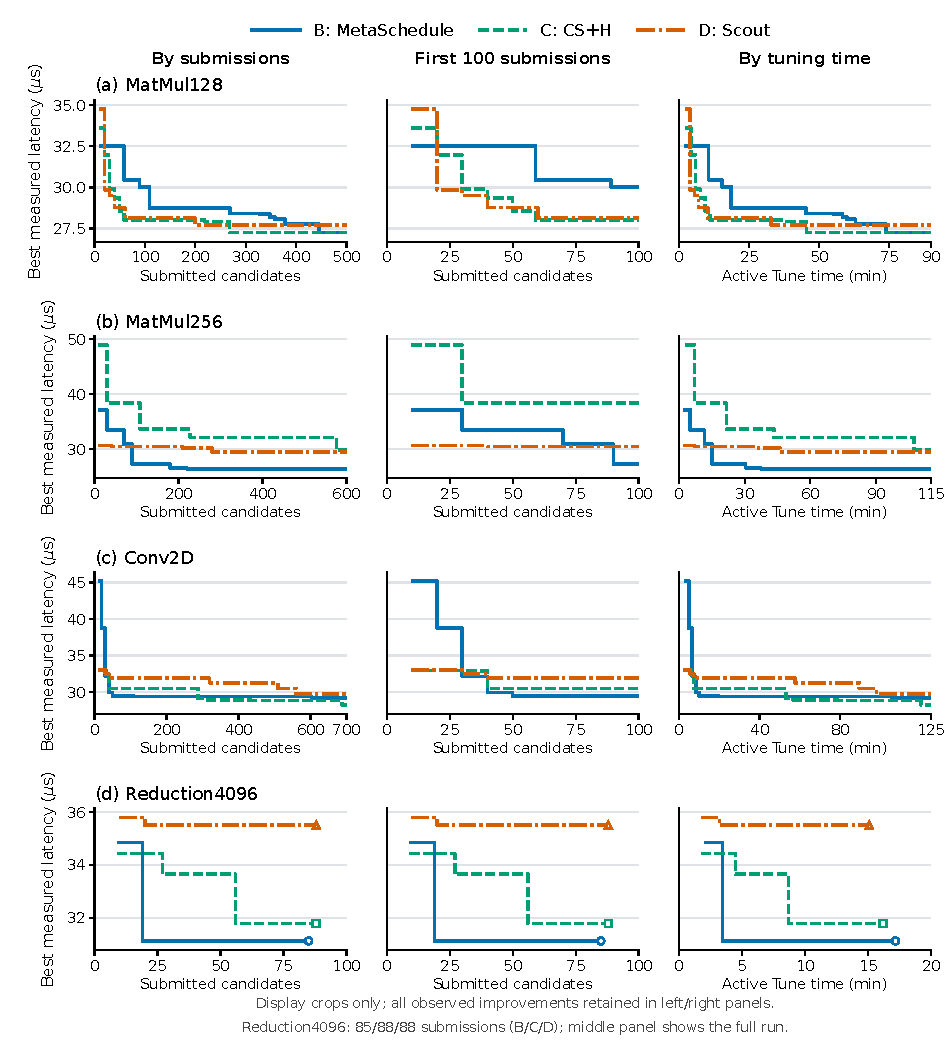
\includegraphics[width=\textwidth]{figures/operator800_20261011_cohort/paper_main_convergence_zoomed/operator800_main_convergence.pdf}
\caption{算子收敛与前 100 次放大。左列依次截至 500/600/700/100 次提交，右列依次截至 90/115/125/20 min，三种方法共用显示范围；左右两列保留全部已观测改善。纵轴为累计最佳延迟。B/C/D 分别为 MetaSchedule、CS+H、完整 Scout。空心点表示实际终点；归约仅 85/88/88 次，中列覆盖完整运行。Conv2D/C 不计暂停与状态重建。单搜索 seed，重测不回填。}
\label{fig:operator800-convergence}
\end{figure*}

\begin{table*}[t]
\centering
\caption{全部运行的收敛位置与统一目标时间，单位为 min。自身最佳位置取完整反馈后的批末；严格、+1\%、+5\% 目标均相对于同算子 B 的搜索终点。NR 表示截至本行总调优时间仍未达到目标。}
\label{tab:operator800-convergence}
\small
\setlength{\tabcolsep}{4pt}
% Generated by experiments/build_operator800_paper_tables.py.
\begin{tabular*}{\textwidth}{@{\extracolsep{\fill}}lrrrrrr@{}}
\toprule
算子 / 配置 & \shortstack{自身最佳\\提交数} & \shortstack{自身最佳\\时间} & \shortstack{严格\\目标} & \shortstack{+1\%\\目标} & \shortstack{+5\%\\目标} & 总调优 \\
\midrule
MatMul128 / B & 446 & 74.08 & 74.08 & 74.08 & 45.37 & 134.01 \\
MatMul128 / C & 268 & 45.65 & NR & 45.65 & 9.39 & 135.21 \\
MatMul128 / D & 200 & 32.84 & NR & NR & 10.29 & 130.31 \\
\midrule
MatMul256 / B & 220 & 37.22 & 37.22 & 30.47 & 15.17 & 136.48 \\
MatMul256 / C & 576 & 107.36 & NR & NR & NR & 150.60 \\
MatMul256 / D & 280 & 46.04 & NR & NR & NR & 132.57 \\
\midrule
Conv2D / B & 603 & 105.57 & 105.57 & 10.01 & 8.36 & 140.23 \\
Conv2D / C & 688 & 120.02 & 53.06 & 53.06 & 7.56 & 139.23 \\
Conv2D / D & 560 & 98.10 & NR & NR & 89.50 & 138.00 \\
\midrule
Reduction / B & 19 & 3.45 & 3.45 & 3.45 & 3.45 & 17.19 \\
Reduction / C & 56 & 8.71 & NR & NR & 8.71 & 16.22 \\
Reduction / D & 20 & 3.23 & NR & NR & NR & 15.11 \\
\bottomrule
\end{tabular*}

\end{table*}

\paragraph{剪枝配置的达标收益}
Conv2D 中，C 在 53.06 min 达到 B 的严格终点目标，B 首次达到该目标需要 105.57 min，因此 C 取得 $1.99\times$ 达标加速，对应耗时减少 49.7\%。C 随后继续改善，在 120.02 min 获得自身最佳观测值 $28.245\,\mu$s。完整提交上限下，C/B 总时间分别为 139.23/140.23 min；提前获得目标性能的收益明显大于跑完全部提交后的总时间差异。

MatMul128 中，C 的终点为 $27.253\,\mu$s，与 B 的 $27.246\,\mu$s 相差约 0.025\%，未满足严格目标；在 +1\% 目标下，C/B 分别需要 45.65/74.08 min，获得 $1.62\times$ 达标加速，耗时减少 38.4\%。在 +5\% 目标下，两者分别需要 9.39/45.37 min。MatMul256/C 则在三个目标下均未达标；Reduction/C 仅达到 +5\% 目标，且晚于 B。这些差异表明剪枝对候选数量的改善尚不能推导为所有负载上的收敛加速。

\paragraph{分级筛选的质量与时间权衡}
D 在四个算子上均未达到严格及 +1\% 目标。MatMul128/D 虽在 32.84 min 获得自身最终最佳值，但其延迟比 B 高约 1.73\%；Conv2D/D 在 +5\% 目标下需要 89.50 min，也晚于 B 的 8.36 min。因此，较早出现自身平台并不表示在相同质量下更快收敛。矩阵乘与卷积的 D 相对 B 总调优时间分别减少 2.76\%、2.87\% 和 1.59\%，但均伴随较差的终点或重测性能；归约的实际提交数还不同，需连同终止位置和程序质量解读。

\FloatBarrier
\subsection{约束剪枝对无效探索的影响}
\label{sec:invalid-exploration}
表~\ref{tab:invalid-exploration} 比较 B/C 的内部生成尝试、\texttt{VerifyGPUCode} 失败和后处理通过率。内部生成次数不等于硬件提交数；通过率以实际通过后处理的数量除以生成次数计算，其他阶段也可能拒绝候选，故不使用一减 Verify 失败率替代。

\begin{table*}[t]
\centering
\caption{约束剪枝对内部候选的影响。每种配置依次列出生成数、Verify 失败数及后处理通过率。$\dagger$：Conv2D/C 为接续运行，原生内部计数包含状态重建期间的工作，不能视为与活动 Tune 时间严格对齐的增量计数。}
\label{tab:invalid-exploration}
\small
\setlength{\tabcolsep}{4pt}
% Generated by experiments/build_operator800_paper_tables.py.
\begin{tabular*}{\textwidth}{@{\extracolsep{\fill}}lrrrrrr@{}}
\toprule
 & \multicolumn{3}{c}{B：MetaSchedule} & \multicolumn{3}{c}{C：CS+H} \\
算子 & 生成数 & Verify 失败 & 通过率 & 生成数 & Verify 失败 & 通过率 \\
\midrule
MatMul128 & 22018 & 17128 & 22.2\% & 7436 & 1950 & 70.3\% \\
MatMul256 & 25529 & 20602 & 19.3\% & 9983 & 4631 & 51.7\% \\
Conv2D$^{\dagger}$ & 19841 & 14890 & 25.0\% & 7463 & 1944 & 71.1\% \\
Reduction & 760 & 0 & 100.0\% & 759 & 0 & 100.0\% \\
\bottomrule
\end{tabular*}

\end{table*}

在 MatMul128 上，C 将生成次数从 22018 减至 7436，减少 66.2\%；Verify 失败从 17128 减至 1950，减少 88.6\%；后处理通过率由 22.2\% 升至 70.3\%。MatMul256 的生成次数和 Verify 失败分别减少 60.9\% 和 77.5\%，通过率由 19.3\% 升至 51.7\%。Conv2D 的原生累计记录同样呈现更少生成与失败、更高通过率的趋势，但含重建工作，应与其活动时间分开使用。Reduction 的基线 Verify 失败已经为零，B/C 通过率均为 100\%，缺少同类非法候选可供剪除。

这些结果支持线程约束前移能减少相关负载的无效内部探索；本组比较尚未分离 CS 与 H 的各自贡献。候选数量变化也不等于 Search 时间同比减少：例如 MatMul128 的 B/C 搜索阶段分别耗时 17.07/17.95 min，额外约束分析和不同搜索轨迹共同影响实际成本。

\subsection{分级筛选与学习代价模型成本}
\label{sec:ga-density}
表~\ref{tab:operator800-model-history} 汇总全部运行的模型反馈历史和评分成本。评分时间包围 \texttt{CostModel::Predict}，包含特征提取、数据整理与预测，不仅是树模型推理；模型更新时间包含特征、验证与重新拟合，是反馈回调的子项。

\begin{table*}[t]
\centering
\caption{学习代价模型与 Draft 的累计成本，时间单位为 s。评分输入按调用累计，可重复包含同一候选；历史样本为实际测量反馈数，更新回调次数含无新增反馈的空批次。$\dagger$：Conv2D/C 的模型评分输入数和评分时间包含状态重建，表中保留原值，不据此计算活动调优期间的 C/D 净节省。}
\label{tab:operator800-model-history}
\label{tab:draft-scoring}
\small
\setlength{\tabcolsep}{4pt}
% Generated by experiments/build_operator800_paper_tables.py.
\begin{tabular*}{\textwidth}{@{\extracolsep{\fill}}lrrrrrr@{}}
\toprule
算子 / 配置 & \shortstack{累计\\样本} & \shortstack{更新回调\\次数} & \shortstack{模型评分\\输入数} & \shortstack{模型评分\\时间} & \shortstack{模型更新\\时间} & \shortstack{Draft\\时间} \\
\midrule
MatMul128 / B & 800 & 81 & 5184 & 27.915 & 22.434 & -- \\
MatMul128 / C & 800 & 81 & 5184 & 27.551 & 25.076 & -- \\
MatMul128 / D & 800 & 80 & 800 & 4.314 & 22.541 & 0.927 \\
\midrule
MatMul256 / B & 800 & 81 & 5184 & 28.240 & 28.428 & -- \\
MatMul256 / C & 800 & 81 & 5184 & 30.941 & 30.582 & -- \\
MatMul256 / D & 800 & 80 & 800 & 4.256 & 28.490 & 0.789 \\
\midrule
Conv2D / B & 800 & 81 & 5184 & 107.516 & 40.204 & -- \\
Conv2D / C$^{\dagger}$ & 800 & 82 & 5248 & 99.787 & 42.743 & -- \\
Conv2D / D & 800 & 80 & 800 & 16.845 & 37.844 & 1.718 \\
\midrule
Reduction / B & 85 & 16 & 1088 & 1.414 & 3.814 & -- \\
Reduction / C & 88 & 16 & 1088 & 1.319 & 3.454 & -- \\
Reduction / D & 88 & 15 & 88 & 0.114 & 3.296 & 0.041 \\
\bottomrule
\end{tabular*}

\end{table*}

MatMul128 和 MatMul256 中，D 将学习模型评分输入数均由 C 的 5184 降至 800，减少 84.6\%；评分时间分别从 27.551/30.941 s 降至 4.314/4.256 s，减少 84.3\%/86.2\%。归约中，评分输入数从 1088 降至 88，评分时间从 1.319 s 降至 0.114 s，减少 91.4\%。对应 Draft 已记录耗时分别为 0.927、0.789 和 0.041 s。这些结果说明解析评分替代高频学习模型调用能够降低评分环节成本。Draft 计时尚未完整覆盖归档排序、候选收集与堆插入，因此不能将两类计时之差直接作为系统净收益。

九组 800 次提交实验均保留 800 个历史样本，归约三组保留 85/88/88 个样本；D 并未减少实际反馈样本量，也未改变非空反馈批次使用累计历史重新拟合的训练策略。归约三组的更新回调数为 16/16/15，其中实际新增反馈批次为 12/12/11。模型更新回调耗时在矩阵乘与卷积中为 22.4--42.7 s，归约中为 3.3--3.8 s。因此，当前证据支持降低评分及相关特征提取工作量，不能据此声称降低模型训练复杂度。

\begin{table*}[t]
\centering
\caption{全部 12 组活动 Tune 阶段成本（min）。测量与反馈包含 runner 调度和数值检查；模型更新包含在回调中，不重复相加。总调优不含 Tune 前准备、独立重测和接续状态重建，归约按实际终止点统计；四舍五入可能造成小计差异。}
\label{tab:operator800-phases}
\small
\setlength{\tabcolsep}{4pt}
% Generated by experiments/build_operator800_paper_tables.py.
\begin{tabular*}{\textwidth}{@{\extracolsep{\fill}}lrrrrrr@{}}
\toprule
算子 / 配置 & 搜索 & 编译 & 测量与反馈 & 回调 & 其他 & 总调优 \\
\midrule
MatMul128 / B & 17.07 & 91.08 & 4.99 & 20.45 & 0.42 & 134.01 \\
MatMul128 / C & 17.95 & 91.37 & 4.97 & 20.49 & 0.42 & 135.21 \\
MatMul128 / D & 16.51 & 87.91 & 5.01 & 20.45 & 0.43 & 130.31 \\
\midrule
MatMul256 / B & 19.40 & 90.99 & 5.15 & 20.55 & 0.39 & 136.48 \\
MatMul256 / C & 23.88 & 100.33 & 5.33 & 20.59 & 0.48 & 150.60 \\
MatMul256 / D & 21.53 & 84.93 & 5.16 & 20.55 & 0.40 & 132.57 \\
\midrule
Conv2D / B & 18.23 & 95.38 & 5.38 & 20.75 & 0.49 & 140.23 \\
Conv2D / C & 18.51 & 94.52 & 4.89 & 20.80 & 0.51 & 139.23 \\
Conv2D / D & 16.96 & 94.37 & 5.47 & 20.71 & 0.48 & 138.00 \\
\midrule
Reduction / B & 0.05 & 13.85 & 0.63 & 2.20 & 0.47 & 17.19 \\
Reduction / C & 0.04 & 12.92 & 0.62 & 2.27 & 0.37 & 16.22 \\
Reduction / D & 0.03 & 11.86 & 0.61 & 2.26 & 0.35 & 15.11 \\
\bottomrule
\end{tabular*}

\end{table*}

作为补充，独立的 32 次提交 MatMul128 初步实验曾比较 GA1/GA4：C 的模型评分输入由 512 增至 1280，D 均为 64；C/D 评分时间从 2.561/0.333 s 变为 6.427/0.330 s。该小预算结果说明内部搜索增密会放大学习模型评分成本，未证明增加代数能够改善最终程序质量，也不与 800 上限的主实验合并计算收益。

\subsection{完整调优成本与实验范围}
\label{sec:cost-and-feedback}
表~\ref{tab:operator800-phases} 将活动 Tune 时间分为互不重叠的阶段。矩阵乘与卷积中，编译是主要成本，耗时为 84.93--100.33 min；搜索为 16.51--23.88 min，反馈回调约为 20.45--20.80 min。归约的编译耗时为 11.86--13.85 min，搜索仅约 0.03--0.05 min。因而，减少数秒至数十秒的评分调用，尚不足以显著改变当前以编译为主的完整预算成本。

\paragraph{证据边界与后续验证}
\label{sec:end-to-end}
上述结论来自单块 GPU、一个搜索 seed 和四个固定形状的 FP32 算子。30 次技术重测不能替代多 seed 搜索，归约提前终止也不能解释为已完成 800 次测量。完整模型调优目前尚无完成的三配置对照，不将单算子结果或中断模型运行作为端到端收益证据。后续需补充多 seed、其他设备、完整模型，以及固定随机探索比例和独立候选池下的排序与保留率实验，以检验分级筛选在程序质量、入围比例和搜索密度之间的权衡。
\FloatBarrier
\endgroup


\section{讨论与相关工作}
\label{sec:related}
Ansor 与 MetaSchedule 分别提供自动搜索框架和基于概率程序的调度空间表达~\cite{ansor,metaschedule}。与将搜索空间整体重构为约束满足问题的 Heron~\cite{heron} 不同，本文以 retrofit 方式在现有 MetaSchedule 流程中注入约束判定，不重建调度空间。本文利用已有线程契约前移判定，不声称所有既有系统均未处理可行性。Pruner 是粗筛（解析评分）组件的直接方法来源~\cite{pruner}；本地集成关注其在现有约束搜索路径下的成本与质量，不能与论文中不同硬件结果直接计算加速比。

当前有四项主要局限。第一，线程规则仅在支持结构上可证明，且相对于基线契约而非无约束硬件空间安全；固定池已覆盖两个有限提案池的提前拒绝 oracle，但未覆盖完整线上轨迹、全部未知结构或其他 shape。第二，单个搜索 seed、每臂 32 次提交不足以证明统计显著性；独立重测为技术重复而非独立搜索样本，最小延迟仍受测量噪声与选择偏差影响。第三，固定池诊断已区分首个失败类别并定位软件流水线 pass，但尚未获得跨形状的安全提前判据；pass 观察时间有嵌套与诊断开销，不能代替正式互斥阶段计时，scheduler 时间也不能冒充完整墙钟。第四，主对照只有单设备、单 seed，模型级（ResNet-18）与更大预算、更多 seed 的实验不完整。

下一阶段在已完成的首因诊断和反事实基础上，区分安全资源剪枝、结构修复与异常快速返回，选择具有证明依据和净收益的前移约束；同时扩展配对 seed 和 32/64 次提交预算，再补标准 Conv2D 与较大 Reduction 对照。正式比较同时报告提交数、finite 数与 Tune 墙钟，候选特有编译失败仍占预算，不只发表全成功运行。目标性能提前固定，未达标运行保留删失信息。双信号通过离线验证后才加入完整在线矩阵。

\subsection{未来工作：绝对排名与父子相对改进}
\label{sec:hypothesis}
本小节是\emph{待实现和验证的研究方案}，不是现有实验证明的贡献。动机是限制单一粗筛偏差在进化和归档中的累积，同时保留低成本评分路径。

对于真实父子关系 $(p,c)$，若原始分数均已知、为正且定义可比，计划引入
\begin{equation}
\Delta_D(p,c)=\log\frac{D(c)+\epsilon}{D(p)+\epsilon},\qquad \epsilon>0.
\end{equation}
绝对分数描述候选本身的预计质量，相对变化描述一次变异的预计改进。不能使用每代独立归一化后的分数计算比值，也不能按 tile 相似性捏造父子谱系。$\Delta_D$ 来自同一个粗筛分数，并非新增实测信息，可能继承其偏差。

拟将固定归档名额分为绝对精英、不同父代或结构组的相对改进候选、随机探索三类。先保留结构多样性对照，再判断相对信号是否提供额外信息。低粗筛分数或 unknown 不作为合法性硬拒；首版每次变异只产生一个子代，不通过大量分支 replay 选择方向；GA 内不调用 XGBoost。

需要注意，对于同一父代 $p$，$\log(D(p)+\epsilon)$ 为常数，按 $\Delta_D(p,c)$ 排序与按 $D(c)$ 排序完全相同。因此必须加入“相同父组配额加子代绝对分数”和“相同父组配额加随机子代”两个对照，先检查入选集合是否实际改变。若组内固定配额下集合相同，不能将收益归因为相对打分的独立信息；跨父组分配改变时还需检验对低分父代的偏好。

验证顺序为：采集完整谱系与候选池；在独立划分上检验 $\Delta_D$ 与真实 $\log(L(p)/L(c))$ 的相关性和改进方向一致率；比较随机、绝对排名、绝对排名加多样性、绝对排名加相对信号及完整组合。先报告池内 Recall@K、regret、覆盖率和新增开销，通过后才开展在线配对。当前不能声称该方案已改善质量、已经避免额外 replay 或具有未经文献核验的独立新颖性。

\section{结论}
本文实现并评估 MetaSchedule 中的剪枝与分级筛选。在 CUDA sm\_86 的 MatMul128/256、标准卷积与大归约上，剪枝（CS+H）减少了无效候选生成，分级筛选降低了学习模型的评分工作量，但完整调优时间的降幅均不足 1%，且除大归约外未呈现一致的质量优势。这说明减少内部搜索工作能否改善实际调优，取决于评分偏差与编译成本所占的比例。后续重点是提高可证明约束的前移覆盖、在固定工作量下检验净成本，并完成 ResNet-18 模型级验证，而非预设加速结论。

\appendix
\section{测量细节与附表}
\label{sec:measurement-details}
本批实验统一使用 TVM \texttt{0.26.dev90}、CUDA 12.6 与 \texttt{sm\_86} 目标，平台为 RTX 3050 Ti Laptop GPU（4 GiB）。搜索 seed 固定为 20261011，每臂 32 submitted、批大小 4、种群 32、探索比例 0.1；MatMul128 分别设置 1 与 4 代 GA，其余为 1 代。代价模型为 XGBoost、warmup 0；D 的入围比例 \texttt{verify\_ratio}=0.25。每个候选在计时前通过独立缓冲的数值检查（与 NumPy FP64 参考比对，rtol=atol=$2\times10^{-4}$）；完整调优时间从 Tune 开始到返回，含 search、builder、runner 与 callback，准备时间单列。

15 次运行、480 次提交均获得有限且数值正确的测量。Windows 上完成测量后的进程退出异常通过 worker 规避处理，未宣称根因修复。表~\ref{tab:single-primary} 报告生成/Verify 与时间，表~\ref{tab:single-ga} 报告 GA 密度下的评分开销，表~\ref{tab:single-targets} 报告全部目标阈值；图~\ref{fig:single-retiming} 给出原 top-1 独立重测的完整分布。

% Auto-generated from audited summary.json; do not edit numeric cells.
% Source SHA256: 32b22c8a529af34f8b22a9bfd7397a15e93341e689830e89ff46a5cdcd1cc663
% Regenerate with experiments/export_single_seed_paper_tables.py.
\begin{table*}[tb]
\centering
\caption{同预算主结果：预先固定一个搜索 seed（20261011），每臂 32 submitted，均得到 32 次有限且正确的测量。B=baseline，C=CS+H，D=CS+H+粗筛。观测最优来自调优数据库；重测固定原 top-1，每臂 30 个技术重复的中位数，不回填调优曲线，也不增加独立搜索 seed。}
\label{tab:single-primary}
\fontsize{9}{11}\selectfont
\setlength{\tabcolsep}{4pt}
\begin{tabular}{llrrrrrr}
\toprule
算子 / GA & 臂 & 生成 & \shortstack{Verify\\失败} & \shortstack{Search\\(s)} & \shortstack{Tune\\(s)} & \shortstack{观测最优\\($\mu$s)} & \shortstack{原 top-1 重测\\中位数 ($\mu$s)} \\
\midrule
MatMul128 / 1 & B & 2018 & 1531 & 105.154 & 790.161 & 34.0845 & 31.7013 \\
 & C & 773 & 231 & 145.273 & 778.711 & 33.6107 & 31.8705 \\
 & D & 732 & 210 & 127.051 & 773.069 & 33.5186 & 34.0597 \\
\midrule
MatMul128 / 4 & B & 3068 & 1952 & 133.155 & 765.013 & 33.0918 & 37.5262 \\
 & C & 1474 & 224 & 140.818 & 817.116 & 35.2377 & 36.1484 \\
 & D & 1535 & 274 & 143.172 & 811.631 & 33.4867 & 35.1035 \\
\midrule
MatMul256 / 1 & B & 2453 & 1966 & 136.738 & 802.983 & 32.8173 & 31.4930 \\
 & C & 1040 & 516 & 172.585 & 867.306 & 50.0943 & 44.1429 \\
 & D & 966 & 451 & 140.925 & 783.873 & 33.8304 & 34.4057 \\
\midrule
Conv / 1 & B & 1958 & 1467 & 119.082 & 794.351 & 34.3407 & 37.7946 \\
 & C & 758 & 199 & 118.814 & 809.308 & 33.7829 & 37.6410 \\
 & D & 757 & 208 & 134.831 & 834.919 & 34.9225 & 37.6904 \\
\midrule
Reduction / 1 & B & 373 & 0 & 1.353 & 665.286 & 35.7334 & 35.9612 \\
 & C & 344 & 0 & 1.376 & 665.380 & 37.2612 & 36.8367 \\
 & D & 359 & 0 & 0.816 & 628.305 & 33.5466 & 32.4199 \\
\bottomrule
\end{tabular}
\end{table*}

% Auto-generated from audited summary.json; do not edit numeric cells.
% Source SHA256: 32b22c8a529af34f8b22a9bfd7397a15e93341e689830e89ff46a5cdcd1cc663
% Regenerate with experiments/export_single_seed_paper_tables.py.
\begin{table*}[tb]
\centering
\caption{MatMul128 的 GA 密度与评分开销：同一搜索 seed，每臂 32 submitted。预测节省与 Tune 减少均比较 C（CS+H）到 D（CS+H+粗筛）；粗筛自身评分和 XGBoost 预测已嵌套于 Search，不能重复加入总 Tune。}
\label{tab:single-ga}
\small
\setlength{\tabcolsep}{4pt}
\begin{tabular}{rrrrrrr}
\toprule
GA & \shortstack{XGB 输入\\C$\to$D} & \shortstack{C 预测\\(s)} & \shortstack{D 预测\\(s)} & \shortstack{预测节省\\(s)} & \shortstack{D 粗筛评分\\(s)} & \shortstack{Tune 减少\\(\%)} \\
\midrule
1 & $512\to64$ & 2.560564 & 0.333087 & 2.227477 & 0.079086 & 0.72 \\
4 & $1280\to64$ & 6.427177 & 0.330386 & 6.096791 & 0.223606 & 0.67 \\
\bottomrule
\end{tabular}
\end{table*}

% Auto-generated from audited summary.json; do not edit numeric cells.
% Source SHA256: 32b22c8a529af34f8b22a9bfd7397a15e93341e689830e89ff46a5cdcd1cc663
% Regenerate with experiments/export_single_seed_paper_tables.py.
\begin{table*}[tb]
\centering
\caption{全部目标阈值的达标提交数 / 完整 Tune 秒数：一个搜索 seed，每臂 32 submitted。NR(截止秒数) 表示预算耗尽仍未达标。MatMul128 的 40/50\,$\mu$s 为预定目标；扩展算子的三档目标为各自 baseline 调优终点的 1/1.01/1.05 倍，属于回顾性描述。整批 callback 完成后才判定达标，不插值，准备时间单列；目标依据调优观测，独立原赢家重测不回填本表。}
\label{tab:single-targets}
\small
\setlength{\tabcolsep}{4pt}
\begin{tabular}{lrrrr}
\toprule
算子 / GA & \shortstack{目标\\($\mu$s)} & \shortstack{B\\提交 / Tune (s)} & \shortstack{C\\提交 / Tune (s)} & \shortstack{D\\提交 / Tune (s)} \\
\midrule
MatMul128 / 1 & 40.0000 & 4 / 128.634 & 4 / 118.522 & 4 / 120.822 \\
 & 50.0000 & 4 / 128.634 & 4 / 118.522 & 4 / 120.822 \\
\midrule
MatMul128 / 4 & 40.0000 & 4 / 113.543 & 24 / 628.530 & 4 / 121.206 \\
 & 50.0000 & 4 / 113.543 & 4 / 126.508 & 4 / 121.206 \\
\midrule
MatMul256 / 1 & 32.8173 & 32 / 802.979 & NR(867.306) & NR(783.873) \\
 & 33.1455 & 28 / 702.860 & NR(867.306) & NR(783.873) \\
 & 34.4582 & 12 / 312.693 & NR(867.306) & 4 / 124.729 \\
\midrule
Conv / 1 & 34.3407 & 4 / 127.076 & 4 / 126.255 & NR(834.919) \\
 & 34.6841 & 4 / 127.076 & 4 / 126.255 & NR(834.919) \\
 & 36.0577 & 4 / 127.076 & 4 / 126.255 & 20 / 554.838 \\
\midrule
Reduction / 1 & 35.7334 & 16 / 338.406 & NR(665.380) & 32 / 628.301 \\
 & 36.0907 & 16 / 338.406 & NR(665.380) & 32 / 628.301 \\
 & 37.5201 & 12 / 263.545 & 4 / 102.552 & 4 / 96.277 \\
\bottomrule
\end{tabular}
\end{table*}


\begin{figure*}[tb]
\centering
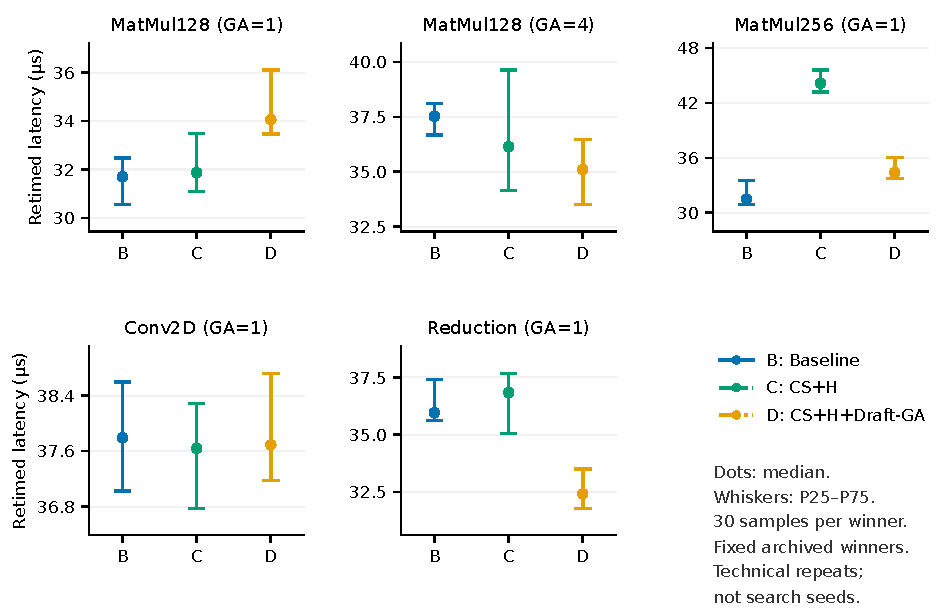
\includegraphics[width=\linewidth]{figures/single_seed_paper_20261010/f5_independent_top1.pdf}
\caption{原 top-1 候选的独立重测延迟分布。每臂 30 个技术重复，中位数用于主文比较；技术重复不增加独立搜索 seed。}
\label{fig:single-retiming}
\end{figure*}

\section{固定候选池与失败路径分析}
\label{sec:frozen-pool}
为分离 H 位置与采样分布变化，历史机制实验在 MatMul128 和固定 target 下采集两个独立提案池，其三条比较路径使用同一历史 DLL；该计时不与本批主实验合并。初始化先通过真实 replay 得到完整决策，在后处理前冻结 trace；随后从基线完整后处理通过的固定父代生成单次变异子代。两个池分别有 64 条完整 trace（63 条唯一，7 个初始合法父代），以及 256 次提案中的 255 条完整 trace（238 条唯一，13 个初始合法父代）；后者另有一次未产生子代，保留记账，不补采样。这不是线上完整 GA 轨迹。

比较关闭 H、回放后 IR H、回放前 trace H 三条路径。第三条路径对所有未拒绝者继续 replay 和 IR H。CS 关闭以保持原始决策，每臂使用新的 Schedule、同一 replay seed 和 target 派生的完整七项 postproc 链。对象恢复重新绑定注册指令，不预先执行 replay。所有候选均有完整基线 oracle，包括 H 提前拒绝者；每个通过者的最终 IR 与采集 oracle 做结构相等检查。热身后轮换三臂顺序计时三轮，重复属于技术重复，不是三个独立搜索 seed。

\begin{table*}[tb]
\centering
\caption{固定完整 trace 池的 CPU 机制 pilot。拒绝/通过为每轮次数，时间为三轮候选路径总时间的中位数；不含采集与启动，不是 GPU 调优墙钟。}
\label{tab:frozen-pool}
\begin{tabular}{llrrrr}
\toprule
完整 trace & 路径 & H 拒绝 & Verify 拒绝 & 通过 & 时间 (s) \\
\midrule
64 & 无 H & 0 & 31 & 33 & 2.620 \\
64 & 回放后 H & 28 & 3 & 33 & 2.700 \\
64 & 回放前 H & 28 & 3 & 33 & 2.516 \\
\midrule
255 & 无 H & 0 & 128 & 127 & 16.328 \\
255 & 回放后 H & 111 & 17 & 127 & 16.152 \\
255 & 回放前 H & 111 & 17 & 127 & 15.758 \\
\bottomrule
\end{tabular}
\end{table*}

两个池均未观察到 H 误拒或 oracle 判定不一致。255 条池的 127 次通过对应 110 条唯一通过 trace；该经验安全证据不等于全空间证明或 GPU 数值正确性认证。该池初始化的 128 条完整 trace 中 H 拒绝 103 条，变异的 127 条中仅拒绝 8 条，不应把总体拦截量归为 GA 收益。64 条池还在独立进程中从原文件复评三轮，通过集合、拒绝位置与最终 IR 仍一致；这验证冻结池可复评，不增加独立采样数。

\begin{figure*}[tb]
\centering
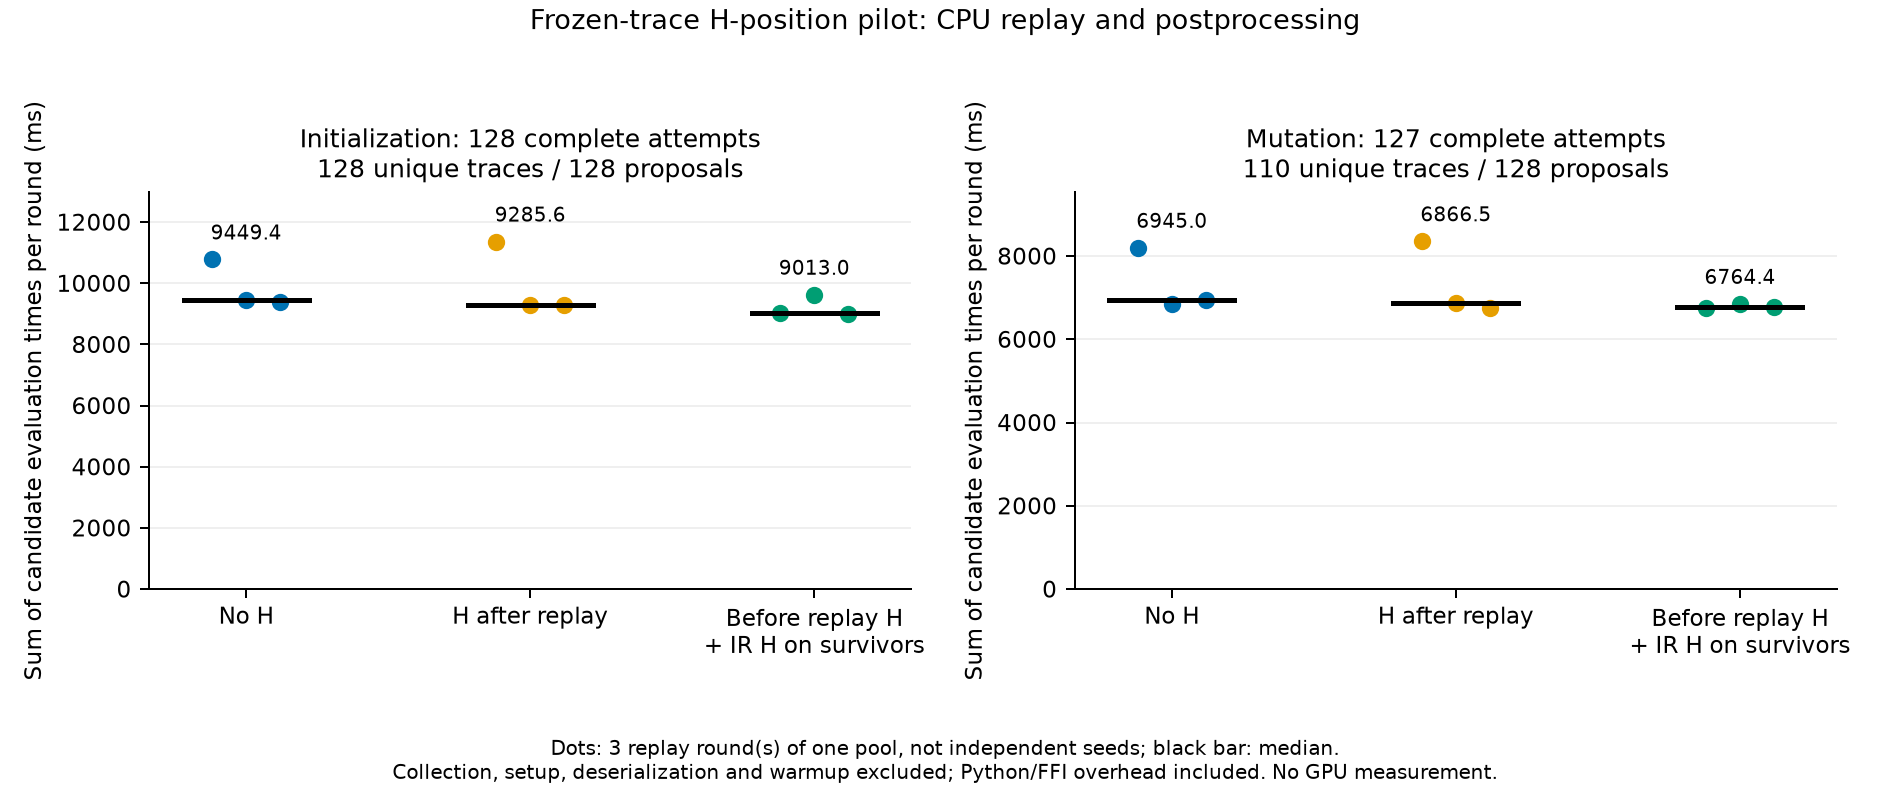
\includegraphics[width=\linewidth]{figures/p1_fixed_pool/pilot02/fixed_pool_round_timing.png}
\caption{255 条完整 trace 池的分阶段 CPU 路径时间。散点为同池三次计时，黑线为中位数；包含 H 检查、replay、postproc 与编排成本，排除采集、对象恢复、热身及结构相等核验。变异阶段的 128 次提案仅产生 127 条完整 trace。}
\label{fig:frozen-pool}
\end{figure*}

回放前 H 的总时间中位数相对无 H 约减少 $4.0\%/3.5\%$，但不能据此宣称稳定端到端收益。尤其在较大池中，111 条早拒者占完整候选的 $43.5\%$，其基线完整处理时间却仅为每轮 $0.609$--$0.691$ s，占基线总时间 $3.64\%$--$3.80\%$；这些候选的 Verify 合计只有 $3.55$--$4.67$ ms。其余 144 条幸存者的 Verify 合计为 $14.86$--$17.36$ s。源码中 Verify 先检查线程契约、失败直接返回，再对剩余候选 lowering，与该现象一致。因此少掉 111 次 Verify 不等于省掉 111 次完整 lowering。

进一步按同一候选 ID 分区可见，H 放行但最终 Verify 失败的 17 条仅占候选的 $6.7\%$，却占基线总路径的 $85.54\%$--$86.14\%$；127 条通过者占 $10.22\%$--$10.66\%$（图~\ref{fig:cost-cohorts}）。其中 8 条失败的 Verify 单条中位耗时为 $1.689$--$1.817$ s，贡献基线总路径的 $84.76\%$--$85.39\%$。这是原始三个技术重复上的成本集中现象，不是已经实现的加速比，也不是针对全部工作负载的总体估计。

\begin{figure*}[tb]
\centering
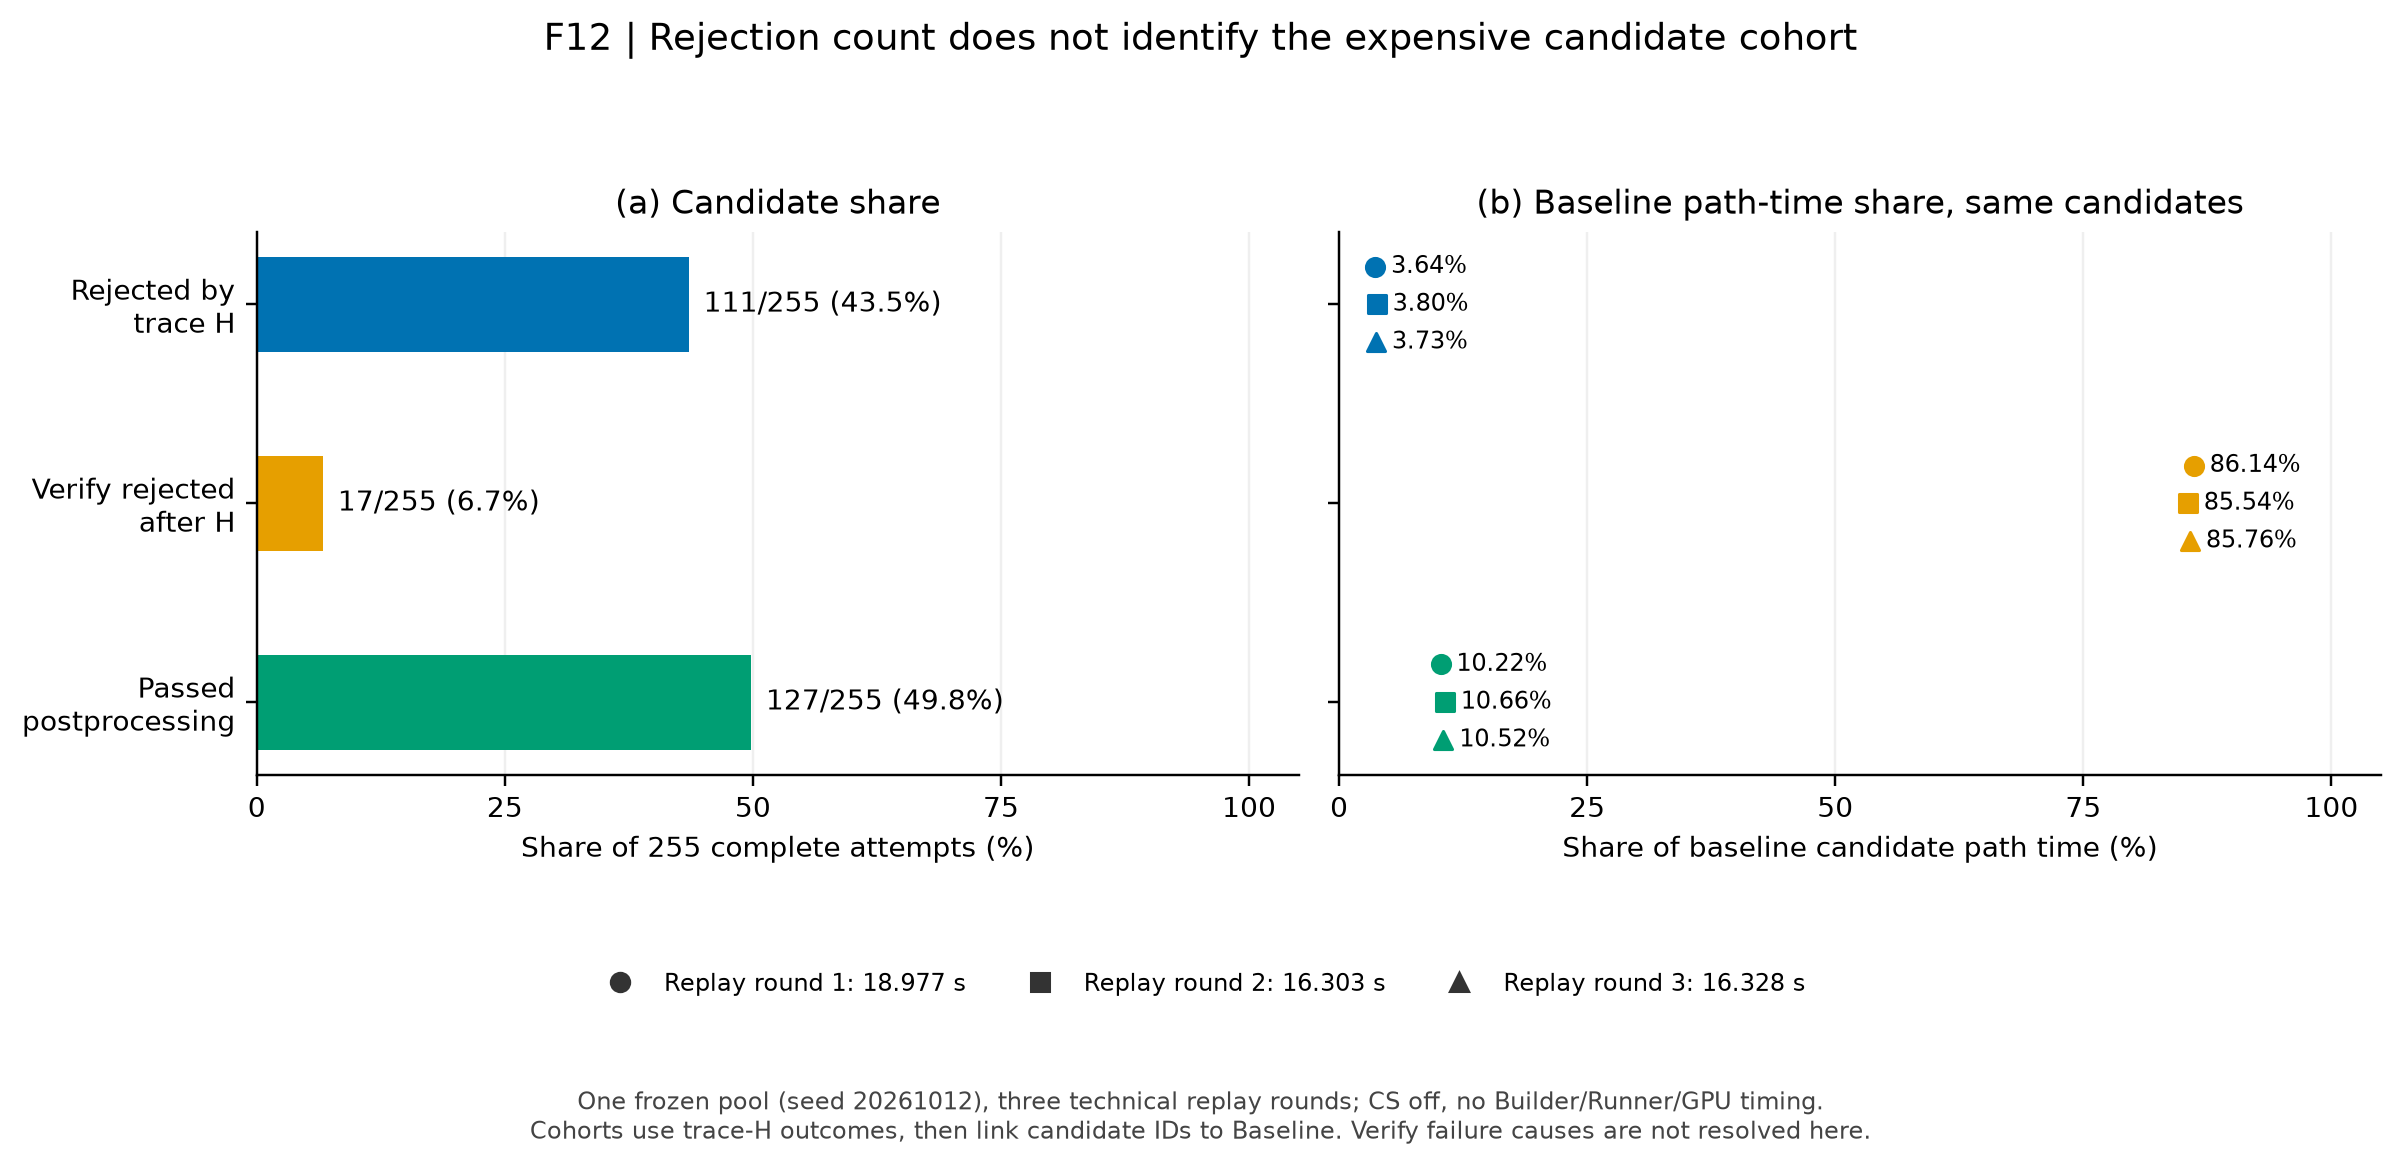
\includegraphics[width=\linewidth]{figures/pilot_mechanism_20261008/f12_fixed_pool_cost_cohorts.png}
\caption{同一固定池的候选数量与基线处理成本。左为按 H 路径确定的三组候选比例，右为回查基线同候选的各轮路径时间占比。17 条残余失败贡献主要成本；三个点为同池技术重复，不是独立搜索 seed，且不含 GPU 测量。}
\label{fig:cost-cohorts}
\end{figure*}

为定位失败，我们仅增加读取 Verify 首个失败类别的只读接口，并编译独立诊断 DLL（SHA256 前缀 \texttt{c2853006ea72}）。在原 255 条完整 trace 上重新执行三条路径，共 765 次判定均与旧 oracle 一致，381 次通过结果的最终 IR 均结构相等。新诊断分类为 111 次线程契约失败、9 次共享内存失败、8 次 lowering 异常及 127 次通过；H 恰好提前拒绝上述 111 次线程失败。随后只对 17 条残余失败进行独立 pass 观察，保持原 PassContext 参数与 lowering 顺序：8 条长尾的最深未闭合 pass 均为 \texttt{s\_tir.InjectSoftwarePipeline}，9 条共享内存失败则完成 lowering 后在资源检查中被拒。诊断计时包含接口与观察器开销，未替换原固定池性能数据；接口只报告首个失败原因，不等于列出了全部违规。

对观察器保存的精确 pass 输入进一步单独调用原软件流水线变换，8 条均重现同一结构错误：流水线阶段注释含 3 项，而实际主体含 4 个块。输入中两个共享内存加载后分别出现归约初始化与更新块，原 3 项注释不再匹配该结构。该证据说明主要长尾的直接触发点是变换契约不一致；它并不排除修复结构后仍存在资源超限。

为区分结构错误与后继资源失败，我们在原 255 条 trace 上观察归约分解前后的 IR，再对上述 8 条分别执行三种反事实：只删除流水线的阶段、顺序和异步阶段注释；将本模板的外层归约因子由 1 改为 2，并将一个可整除的内层因子减半以保持乘积；在原归约后处理之前显式将零初始化提到带注释的单位循环外。原始对照的 255 次状态与首个失败原因均不变，127 次通过结果与原 oracle 的 IR 结构相等。8 条原候选均在 \texttt{RewriteReductionBlock} 前含 3 个直接主体项，之后变为 4 项，而注释保持 3 项；改分块和外提初始化两种干预使所观察主体保持 3 项。这里的直接主体计数仅用于本批归因，不是镜像所有 lowering 变换的通用剪枝判据。

\begin{table*}[tb]
\centering
\caption{同一批 8 条 lowering 失败候选的反事实。三种修改均消除了流水线异常，但不一定消除后继共享内存超限；数量不是独立搜索 seed。}
\label{tab:pipeline-counterfactual}
\begin{tabular}{lrrr}
\toprule
干预 & lowering 异常 & shared 超限 & 完整后处理通过 \\
\midrule
原始候选 & 8 & 0 & 0 \\
关闭流水线注释 & 0 & 7 & 1 \\
外层因子 $1\to2$，乘积不变 & 0 & 8 & 0 \\
零初始化外提 & 0 & 8 & 0 \\
\bottomrule
\end{tabular}
\end{table*}

表~\ref{tab:pipeline-counterfactual} 中唯一通过者为关闭流水线后的 \texttt{mutation-0037}。该程序在同一 RTX 3050 Ti Laptop GPU 上经真实 CUDA 编译，使用三组正态随机输入、一组均匀随机输入、单位矩阵与零矩阵两类结构化输入，并分别以 NaN 和常数初始化输出，共 12 次数值检查均通过。参考为独立 NumPy FP64 矩阵乘，绝对与相对容差均为 $2\times10^{-4}$；最大绝对误差为 $1.979\times10^{-5}$。这是单个修复程序的正确性证据，不是性能测量或通用修复证明。另有单位长度、短于流水线阶段数及动态短循环三项原生变换测试通过，因此不能按短循环长度直接扩展硬筛。

这些结果要求将“当前编译契约不兼容”与“硬件资源不可行”分开。早拒该结构可以避免已知异常路径，却不能被解释为排除了所有潜在好解；若引入修复，需同时提供使用相同修复的基线，才能将修复收益与 CS/H 收益分离。保持流水线的两种修复仍全部受到共享内存限制，后续应验证可靠资源界或限定结构的前置检查，而非仅以异常消失作为验收。

这一结果提示应按\emph{剩余无效工作的成本}而非单纯拒绝比例选择扩展约束。初始化完整决策已在采集时支付首次 replay，两个池的采集总成本分别为 3.621/21.958 s，启动成本为 90.644/84.497 s，均另列。故上述前移收益仅属于完整决策的复评路径，不能直接外推为线上初始化跳过首次 replay，也不构成新增 GPU 性能结果。


\section{数据与复现实验索引}
\raggedright
本批主实验协议和原始结果位于\\
\path{experiments/results/paper_v1/single_seed_20261010/}。
其中 \path{protocol.json} 冻结 seed、版本、开关、顺序、预算及阈值；各运行目录保存数据库、\path{result.json}、逐批计时与数值检查，\path{retiming/} 保存固定原赢家重测和退出诊断。完成情况与原始记录索引见该目录中的 \path{COMPLETION.json}。

汇总数值和输入/输出哈希分别见\\
\path{papers/figures/single_seed_20261010/summary.json}、\\
\path{papers/figures/single_seed_20261010/manifest.json}。\\
论文图及其输入哈希见\\
\path{papers/figures/single_seed_paper_20261010/manifest.json}。\\
执行、独立重测和分析脚本分别为\\
\path{experiments/run_single_seed_study.py}、\\
\path{experiments/remeasure_top1.py} 与\\
\path{experiments/report_single_seed_study.py}。



历史 16 次提交 pilot 的执行计划见\\
\path{experiments/EXPERIMENT_PLAN_20261008.md}。
这些历史结果使用不同版本，仅作补充，不合并为本批搜索重复；目录如下：
\begin{itemize}[leftmargin=1.6em]
\item \path{experiments/results/paper_v1/e8_convergence_small/seed20260931/}
\item \path{experiments/results/paper_v1/e10_seedpair/seed20260932/}
\end{itemize}
历史诊断保存在 \path{experiments/results/paper_v1/} 下：
\begin{itemize}[leftmargin=1.6em]
\item 安全性：\path{e1_cs_safety/database_audit.json}。
\item 排序质量：\path{e2_topk_recall/} 目录中的\\
\path{pruner_draft_topk_v1_1_p1_trained.json}。
\end{itemize}
成图输入、哈希与计时口径见 \path{papers/figures/pilot_20261008/manifest.json}。这些本地路径用于研究复现，不代替最终投稿需要的公开 artifact 地址。

固定池记录位于以下目录：\\
\path{experiments/results/paper_v1/p1_fixed_pool/}。

其中 \path{pilot01/}、\path{pilot02/} 保存完整池与逐条评估，
\path{pilot01_replay01/} 保存独立进程复评。驱动分别为
\path{experiments/fixed_trace_pool.py} 与 \path{experiments/replay_fixed_trace_pool.py}；
图和成本分区的 manifest 位于 \path{papers/figures/p1_fixed_pool/} 下对应池目录。

成本分组补充图及原始输入哈希见\\
\path{papers/figures/pilot_mechanism_20261008/manifest.json}。
诊断接口构建、测试、原池一致性检查和 pass 轨迹位于\\
\path{experiments/results/paper_v1/p1_verify_diagnostics/}。

诊断脚本为\\
\path{experiments/diagnose_fixed_trace_pool.py}。



\begin{thebibliography}{9}
\raggedright
% GB/T 7714 格式；投稿前从 DOI 复核作者列表与页码。
\bibitem{halide}
RAGAN-KELLEY J, BARNES C, ADAMS A, et al. Halide: A Language and Compiler for Optimizing Parallelism, Locality, and Recomputation in Image Processing Pipelines[C]//Proceedings of the 34th ACM SIGPLAN Conference on Programming Language Design and Implementation (PLDI'13). 2013: 519--530.

\bibitem{tvm}
CHEN T, MOREAU T, JIANG Z, et al. TVM: An Automated End-to-End Optimizing Compiler for Deep Learning[C]//Proceedings of the 13th USENIX Symposium on Operating Systems Design and Implementation (OSDI'18). 2018: 578--594.

\bibitem{tiramisu}
BAGHDADI R, RAY J, ROMMEL M B, et al. Tiramisu: A Polyhedral Compiler for Expressing Fast and Portable Code[C]//Proceedings of the 2019 IEEE/ACM International Symposium on Code Generation and Optimization (CGO'19). 2019: 193--205.

\bibitem{triton}
TILLET P, KUNG H T, COX D. Triton: An Intermediate Language and Compiler for Tiled Neural Network Computations[C]//Proceedings of the 3rd ACM SIGPLAN International Workshop on Machine Learning and Programming Languages (MAPL'19). 2019: 10--19.

\bibitem{ansor}
ZHENG L, JIA C, SUN M, et al. Ansor: Generating High-Performance Tensor Programs for Deep Learning[C]//Proceedings of the 14th USENIX Symposium on Operating Systems Design and Implementation (OSDI'20). 2020: 863--879.

\bibitem{metaschedule}
SHAO J, ZHOU X, FENG S, et al. Tensor Program Optimization with Probabilistic Programs[C]//Advances in Neural Information Processing Systems 35 (NeurIPS'22). 2022: 35783--35796.

\bibitem{pruner}
QIAO L, SHI J, HAO X, et al. Pruner: A Draft-then-Verify Exploration Mechanism to Accelerate Tensor Program Tuning[C]//Proceedings of the 30th ACM International Conference on Architectural Support for Programming Languages and Operating Systems (ASPLOS'25), Volume 2. 2025: 949--965. DOI:10.1145/3676641.3716269.

\bibitem{heron}
BI J, GUO Q, LI X, et al. Heron: Automatically Constrained High-Performance Library Generation for Deep Learning Accelerators[C]//Proceedings of the 28th ACM International Conference on Architectural Support for Programming Languages and Operating Systems (ASPLOS'23), Volume 3. 2023: 314--328.
\end{thebibliography}
\end{document}
